\section{On Prior-Data Conflict in Predictive Bernoulli Inferences}
\label{sec:isipta11}

This section reproduces the work
``On Prior-Data Conflict in Predictive Bernoulli Inferences'',
published as a peer-reviewed contribution to
\emph{ISIPTA'11: Proceedings of the Seventh International Symposium on
Imprecise Probabilities: Theories and Applications} \parencite{Walter2011a}.
As such, it is reproduced here almost verbatim,
except for some minor shortenings, especially in the Introduction (Section~\ref{sec:isipta11-intro}),
and the addition of some comments and footnotes linking this work to other parts of this thesis.
Furthermore, the notation was changed slightly to assure consistency with the rest of the material presented in this thesis.
Specifically, the success probability in Bernoulli trials is denoted by $\theta$ instead of $p$.

%***with Frank's weighting model!***
\subsubsection*{Abstract}
%***abstract***

By its capability to deal with the multidimensional nature of
uncertainty, imprecise probability provides a powerful methodology
to sensibly handle \pdc\ in Bayesian inference. When there is
strong conflict between sample observations and prior knowledge, the posterior model should be more imprecise
than in the situation of mutual agreement or compatibility. Focusing
presentation on the prototypical example of Bernoulli
trials, we discuss the ability of different approaches to deal with \pdc.

We study a generalised Bayesian setting, including Walley's Imprecise Beta-Binomial model
and his extension to handle prior data conflict (called pdc-IBBM here).
We investigate alternative shapes of prior parameter sets, chosen in a way that shows improved
behaviour in the case of \pdc\ and their influence on the posterior predictive distribution.
Thereafter we present a new approach, consisting of an
imprecise weighting of two originally separate inferences, one of which is based on an informative
imprecise prior, whereas the other one is based on an uninformative imprecise prior. This approach
deals with \pdc\ in a fascinating way.
%***end of abstract***

\subsection{Introduction}
\label{sec:isipta11-intro}

Imprecise probability has shown to be a
powerful methodology to cope with the multidimensional nature of
uncertainty (see the discussion in Sections~\ref{sec:ip-intro} and \ref{sec:motivation}).
Imprecision allows the quality of information, on which probability statements are
based, to be modeled. Well supported knowledge is expressed by comparatively
precise models, while highly imprecise (or even vacuous) models reflect scarce (or no) knowledge
on probabilities. This flexible, multidimensional perspective on uncertainty
modeling has intensively been utilized in generalised Bayesian
inference to overcome the criticism of the arbitrariness of
the choice of single prior distributions in traditional Bayesian inference.%
\footnote{%See the basic discussion of the Bayesian approach to statistical inference in Section~\ref{sec:bayes-inference},
This criticism, subsumed by \textcite[\S 5]{1991:walley} as the ``dogma of precision'',
is discussed more detailed in Section~\ref{sec:motivation:bayesian}.}
In addition, only imprecise probability models react reliably to the presence of
\pdc, i.e.\ situations  where ``the prior [places] its mass primarily on
distributions in the sampling model for which the observed data is
surprising'' \parencite[p.~894]{2006:evans}. Lower and upper probabilities%
\footnote{See Section~\ref{sec:ip-main} for a short exposition of lower and upper previsions,
and related mathematical tools for handling uncertainty in statistical inference.}
allow a specific reaction to \pdc, and offer reasonable inferences if the analyst wishes to
stick to his prior assumptions: starting with the same level of ambiguity in the prior
specification, wide posterior intervals can
reflect conflict between prior and data, while
no \pdc\ will lead to narrow intervals.%
\footnote{See the discussions in Sections~\ref{sec:motivation:pdc} and \ref{sec:pdc-sensitivity},
and the ***work*** on \pdc\ in Section~\ref{sec:jstp}.}
Ideally, the model could provide an extra `bonus' of precision if prior %specifications had been `spot on'.
assumptions are very strongly supported by the data.
Such a model would have the advantage
of (relatively) precise answers when the data confirm prior assumptions,
while still rendering more cautionary answers in the case of \pdc,
thus leading to cautious inferences if, and only if, caution is needed.

Although \textcite[p.~6]{1991:walley} explicitly emphasizes this possibility to
express prior-data conflict as one of the main motivations for imprecise probability,
it has received surprisingly little attention. Rare exceptions include two short sections in \textcite[p.~6 and \S 5.4]{1991:walley}
and the papers by \textcite{1991:pericchi}, \textcite{1994:coolen} and
\textcite{2005:whitcomb}. The popular IDM \parencite{1996:walley::idm, 2009:bernard}
and its generalisation to exponential families \parencite{2005:quaeghebeurcooman} do not reflect prior-data conflict.
\textcite{Walter2009a} used the basic ideas of \textcite[\S 5.4]{1991:walley} to extend the approach of
\textcite{2005:quaeghebeurcooman} to models that show sensitivity to \pdc.

In this ***paper***, a deeper investigation of the issue of \pdc\ is undertaken,
focusing on the prototypic special case of predictive inference in Bernoulli trials:%
\footnote{See also the discussion of the Beta-Binomial model in Section~\ref{sec:beta-binom},
and the imprecise Dirichlet-Multinomial model discussed in several examples in Section~\ref{sec:jstp}.}
We are interested in the posterior predictive
probability for the event that a future Bernoulli random quantity
will have the value $1$, also called a `success'. This event is not
explicitly included in the notation, i.e.\ we simply denote its lower
and upper probabilities by $\Pl$ and $\Pu$, respectively. This future Bernoulli random
quantity is assumed to be exchangeable with the Bernoulli random
quantities whose observations are summarised in the data, consisting
of the number $n$ of observations and the number $s$ of these that are
successes. In our analysis of this model, we
will often consider $s$ as a a real-valued observation in $[0,n]$,
keeping in mind that in reality it can only take on
integer values, but the continuous representation is convenient for
our discussions, in particular in our predictive probability plots (PPP),
where for given $n$, $\Pl$ and $\Pu$ are discussed as functions of $s$.

\medskip

Section~\ref{sec:ibbm-framework} describes a general framework for
generalised Bayesian inference in this setting. The method presented in \textcite[\S 5.4.3]{1991:walley},
called `pdc-IBBM' in this paper, is considered in detail in Section~\ref{sec:ibbm-walley}
and we show that its reaction to \pdc\ can be improved
by suitable modifications of the underlying imprecise
priors. A basic proposal along these lines is discussed in
Section~\ref{sec:othershapes}, with further alternatives
sketched in Section~\ref{sec:ibbm-resume}.
Section~\ref{sec:weightedinf} addresses the problem of \pdc\ from a
completely different angle. There, we combine two originally separate
inferences, one based on an informative imprecise prior and one
on an uninformative imprecise prior, by an imprecise weighting
scheme. The ***paper*** concludes with a brief comparison of the different
approaches in Section~\ref{sec:insights}.


\subsection{Imprecise Beta-Binomial Models}
\label{sec:ibbm}

\subsubsection{The Framework}
\label{sec:ibbm-framework}

%***change notation for success probability from $p$ to $\theta$!!!***

The traditional Bayesian approach for our basic problem is the Beta-Binominal model, which expresses prior
beliefs about the probability $\theta$ of observing a `success' by a Beta
distribution. With\footnote{Our notation relates to
Walley's \parencite*{1991:walley} as $\nz \leftrightarrow s_0$, $\yz \leftrightarrow t_0$.}
$f(\theta\mid\nz, \yz) \propto \theta^{\nz\yz -1} (1-\theta)^{\nz(1-\yz)-1}$,
$\yz = \E[\theta\mid\nz,\yz]$ can be interpreted as prior guess of
$\theta$, while $\nz$ governs the concentration of
probability mass around $\yz$, also known as `pseudo counts' or
`prior strength'.\footnote{As in previous parts of the thesis, ${}\uz$ denotes prior parameters; ${}\un$ posterior parameters.}
These denominations are due to the
role of $\nz$ in the update step: With $s$ successes in $n$ draws observed, the
posterior parameters are\footnote{Compare to Section~\ref{sec:regularconjugates},
Equation~\eqref{eq:canonicalupdate}:
the model is prototypic for conjugate Bayesian
analysis in canonical exponential families, for which updating
of the parameters $\nz$ and $\yz$ can be
written as \eqref{equ:update-nn-yn-precise}.} %\vspace*{-1.3ex}
\begin{align}\label{equ:update-nn-yn-precise}
%\nn &= \nz + n, & \yn &= \frac{\nz}{\nz + n}\,\yz + \frac{n}{\nz + n}\, \frac{s}{n}.
\nn &= \nz + n, & \yn &= \frac{\nz\yz + s}{\nz + n}\,.
\end{align}
Thus $\yn$ is a weighted average of the prior parameter $\yz$ and
the sample proportion $s/n$, and potential prior data conflict is simply averaged out.

Overcoming the dogma of precision, formulating generalised Bayes
updating in this setting is straightforward. By Walley's Generalised
Bayes Rule \parencite[\S 6]{1991:walley}%
\footnote{For more details on the Generalised Bayes' Rule and the generalised Bayesian inference procedure,
see Sections~\ref{sec:gbr} and \ref{sec:imprecisebayes}, respectively.}
the imprecise prior $\MZ$, described by convex sets of precise prior distributions,
is updated to the imprecise posterior $\MN$ obtained by updating $\MZ$ element-wise.
In particular, the convenient conjugate analysis used above can be extended:%
\footnote{See the discussion of the general framework for generalised Bayesian inference
based on sets of conjugate priors in Section~\ref{sec:basicsetting}.}
One specifies a prior parameter set
$\PZ$ of $(\nz,\yz)$ values and takes as imprecise
prior the set $\MZ$ consisting of  all convex mixtures of Beta
priors with $(\nz, \yz) \in \PZ$. In this sense, the set of Beta
priors corresponding to $\PZ$ gives the set of extreme points for
the actual convex set of priors $\MZ$. Updating $\MZ$ with the
Generalised Bayes' Rule results in the convex set $\MN$ of posterior
distributions, that conveniently can be obtained by taking the
convex hull of the set of Beta posteriors, which in turn are defined
by the set of updated parameters
$\PN = \{(\nn,\yn) \mid (\nz, \yz) \in \PZ\}$.
This relationship between the sets $\PZ$ and $\PN$ and the sets $\MZ$
and $\MN$ will allow us to discuss different models $\MZ$ and $\MN$ by depicting
the corresponding parameter sets $\PZ$ and $\PN$. When interpreting our results,
care will be needed with respect to convexity. Although
$\MZ$ and $\MN$ are convex, the parameter sets $\PZ$ and $\PN$
generating them need not necessarily be so. %convex.
Indeed, convexity of the parameter set is not necessarily preserved in the update
step: Convexity of $\PZ$ does not imply convexity of $\PN$.

Throughout, we are interested in the posterior predictive
probability $[\Pl,\Pu]$ for the event that a
future draw is a success. In the Beta-Bernoulli model, this
probability is equal to $\yn$, and we get\footnote{%
\textcite{2005:quaeghebeurcooman}, \textcite{Walter2009a}, and \textcite{Walter2007a} use the prototypical character of
(\ref{equ:update-nn-yn-precise}) underlying (\ref{equ:General-Pl}) and
(\ref{equ:General-Pu}) to generalise this inference to models based on canonical exponential families.
See Section~\ref{sec:generalmodel} and \ref{sec:jstp}. ***leave this out here??***}
%
\begin{align}
\Pl = \ynl &:= \min_{\PN} \yn = \min_{\PZ} \frac{\nz\yz + s}{\nz +n}\,, \label{equ:General-Pl}\\
%           & = \min_{\nz \in [\nzl, \nzu]} \frac{\nz\yzl + s}{\nz +n} & &\text{and} \nonumber\\
\Pu = \ynu &:= \max_{\PN} \yn = \max_{\PZ} \frac{\nz\yz + s}{\nz +n}\,. \label{equ:General-Pu}
%           & = \max_{\nz \in [\nzl, \nzu]} \frac{\nz\yzu + s}{\nz +n}. \nonumber
\end{align}
%\begin{align*}
%\Pl(S^* = 1\mid s) &= \min_{(\nn, \yn) \in \PN} \yn \quad \text{and}\\
%\Pu(S^* = 1\mid s) &= \max_{(\nn, \yn) \in \PN} \yn.
%\end{align*}
%$\Pl(S^* = 1\mid s) = \min_{(\nn, \yn) \in \PN} \yn$ and
%$\Pu(S^* = 1\mid s) = \max_{(\nn, \yn) \in \PN} \yn$.


\subsubsection{Walley's pdc-IBBM}
\label{sec:ibbm-walley}

Special imprecise probability models are now obtained by specific
choices of $\PZ$. If one fixes $\nz$ and varies $\yz$ in an interval $[\yzl,\yzu]$,
Walley's \parencite*[\S 5.3]{1991:walley} model with learning parameter $\nz$ is obtained, which typically
is used in its near-ignorance form $[\yzl, \yzu] \to (0,1)$,
denoted as the imprecise Beta (Binomal/Bernoulli) model (IBBM)%
\footnote{We use `IBBM' also for the model with prior information.},
which is a special case of the popular Imprecise Dirichlet (Multinomial) Model
\parencite{1996:walley::idm,1999:walleybernard}. Unfortunately, in this basic form with fixed $\nz$, the model is
insensitive to prior-data conflict \parencite[p.~263]{Walter2009a} ****.
\textcite[\S 5.4]{1991:walley} therefore generalised this
model by additionally varying $\nz$. In his extended model,
called \emph{pdc-IBBM} in this ***paper***, the set of priors is defined via the
set of prior parameters $\PZ = [\nzl, \nzu] \times [\yzl, \yzu]$,
being a two-dimensional interval, or a rectangle set.
Studying inference in this model, it is important to note that the set of posterior parameters
%$\PN = \{(\nn,\yn) \mid [\nzl, \nzu] \times [\yzl, \yzu]\}$
%$\PN = \{(\nn,\yn) \mid (\nz, \yz) \in \PZero\}$ defining the set
%of ***vertex*** posterior distributions is not rectangular anymore.
$\PN$ is not rectangular anymore. The resulting shapes are illustrated in Figure~\ref{fig:spot-banana}: For the
prior set $\PZ = [1, 5 ] \times  [0.4, 0.7]$---thus assuming a priori the
fraction of successes to be between 40\% and 70\% and rating these assumptions
with at least $1$ and at most $5$ pseudo observations---the resulting posterior parameter sets $\PN$
are shown for data consisting of 3 successes in 6 draws (left) and with all 6 draws successes (right). %***TPDA***. On the right, ***PDC***.
We call the left shape \emph{spotlight}, and the right shape
\emph{banana}. In both graphs, the elements of $\PN$ yielding
%the minimal and maximal $\yn$, $\ynl = \LE[p\mid s]$ and $\ynu = \UE[p\mid s]$,
$\ynl$ and $\ynu$, and thus $\Pl$ and $\Pu$,
are marked with a circle.

%\begin{verbatim}
\begin{figure}%[t]
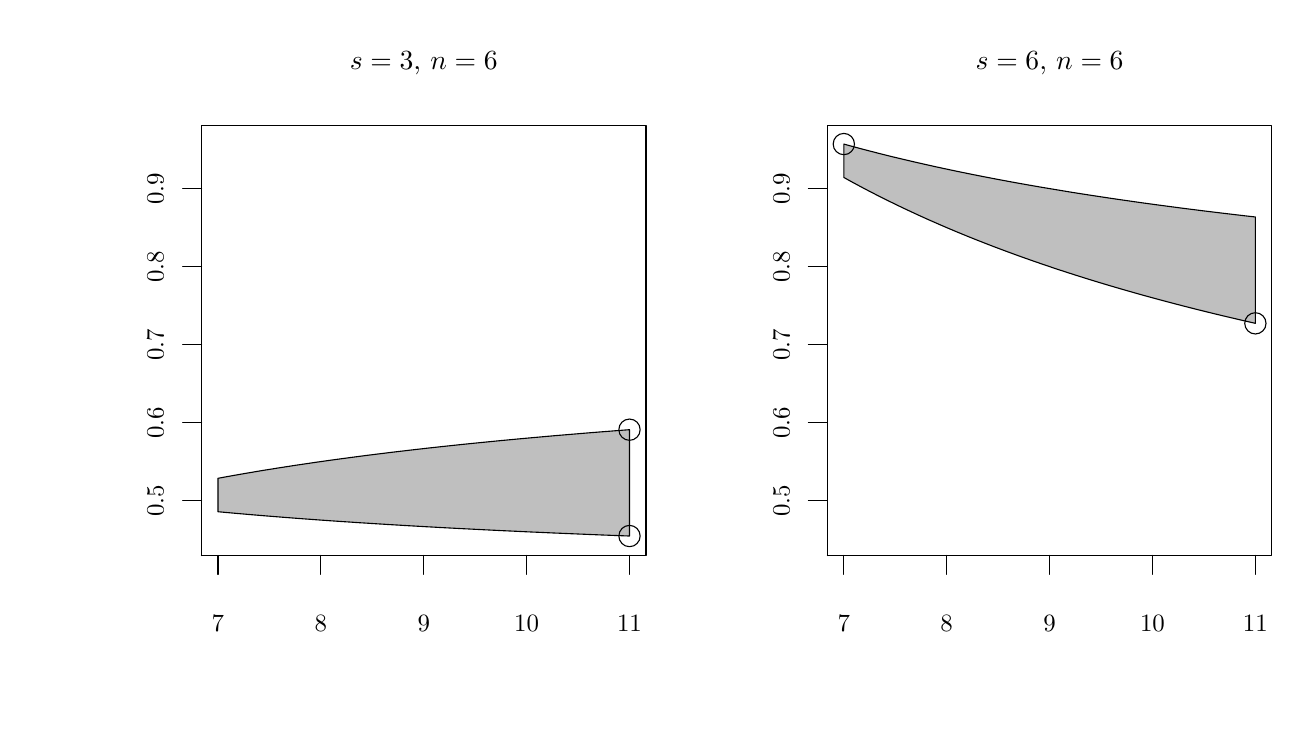
\begin{tikzpicture}
%\pgftransformscale{0.475}
\pgftransformscale{0.04}
%\include{simpleEx.tex}
% Created by tikzDevice version 0.5.0 on 2011-02-28 18:34:50
\begin{scope}
\path[clip] (  0.00,  0.00) rectangle (397.48,216.81);
\definecolor[named]{fillColor}{rgb}{0.88,0.08,0.52}
\definecolor[named]{drawColor}{rgb}{0.00,0.00,0.00}

\draw[color=drawColor,line cap=round,line join=round,fill opacity=0.00,] ( 60.43, 49.20) -- (191.11, 49.20);

\draw[color=drawColor,line cap=round,line join=round,fill opacity=0.00,] ( 60.43, 49.20) -- ( 60.43, 43.20);

\draw[color=drawColor,line cap=round,line join=round,fill opacity=0.00,] ( 93.10, 49.20) -- ( 93.10, 43.20);

\draw[color=drawColor,line cap=round,line join=round,fill opacity=0.00,] (125.77, 49.20) -- (125.77, 43.20);

\draw[color=drawColor,line cap=round,line join=round,fill opacity=0.00,] (158.44, 49.20) -- (158.44, 43.20);

\draw[color=drawColor,line cap=round,line join=round,fill opacity=0.00,] (191.11, 49.20) -- (191.11, 43.20);

\node[color=drawColor,anchor=base,inner sep=0pt, outer sep=0pt, scale=  0.90] at ( 60.43, 25.20) {7%
};

\node[color=drawColor,anchor=base,inner sep=0pt, outer sep=0pt, scale=  0.90] at ( 93.10, 25.20) {8%
};

\node[color=drawColor,anchor=base,inner sep=0pt, outer sep=0pt, scale=  0.90] at (125.77, 25.20) {9%
};

\node[color=drawColor,anchor=base,inner sep=0pt, outer sep=0pt, scale=  0.90] at (158.44, 25.20) {10%
};

\node[color=drawColor,anchor=base,inner sep=0pt, outer sep=0pt, scale=  0.90] at (191.11, 25.20) {11%
};

\draw[color=drawColor,line cap=round,line join=round,fill opacity=0.00,] ( 55.20, 66.64) -- ( 55.20,165.70);

\draw[color=drawColor,line cap=round,line join=round,fill opacity=0.00,] ( 55.20, 66.64) -- ( 49.20, 66.64);

\draw[color=drawColor,line cap=round,line join=round,fill opacity=0.00,] ( 55.20, 91.40) -- ( 49.20, 91.40);

\draw[color=drawColor,line cap=round,line join=round,fill opacity=0.00,] ( 55.20,116.17) -- ( 49.20,116.17);

\draw[color=drawColor,line cap=round,line join=round,fill opacity=0.00,] ( 55.20,140.93) -- ( 49.20,140.93);

\draw[color=drawColor,line cap=round,line join=round,fill opacity=0.00,] ( 55.20,165.70) -- ( 49.20,165.70);

\node[rotate= 90.00,color=drawColor,anchor=base,inner sep=0pt, outer sep=0pt, scale=  0.90] at ( 43.20, 66.64) {0.5%
};

\node[rotate= 90.00,color=drawColor,anchor=base,inner sep=0pt, outer sep=0pt, scale=  0.90] at ( 43.20, 91.40) {0.6%
};

\node[rotate= 90.00,color=drawColor,anchor=base,inner sep=0pt, outer sep=0pt, scale=  0.90] at ( 43.20,116.17) {0.7%
};

\node[rotate= 90.00,color=drawColor,anchor=base,inner sep=0pt, outer sep=0pt, scale=  0.90] at ( 43.20,140.93) {0.8%
};

\node[rotate= 90.00,color=drawColor,anchor=base,inner sep=0pt, outer sep=0pt, scale=  0.90] at ( 43.20,165.70) {0.9%
};

\draw[color=drawColor,line cap=round,line join=round,fill opacity=0.00,] ( 55.20, 49.20) --
	(196.34, 49.20) --
	(196.34,185.61) --
	( 55.20,185.61) --
	( 55.20, 49.20);
\end{scope}
\begin{scope}
\path[clip] (  0.00,  0.00) rectangle (198.74,216.81);
\definecolor[named]{fillColor}{rgb}{0.88,0.08,0.52}
\definecolor[named]{drawColor}{rgb}{0.00,0.00,0.00}

\node[color=drawColor,anchor=base,inner sep=0pt, outer sep=0pt, scale=  1.00] at (125.77,  1.20) {$\nn$%
};

\node[rotate= 90.00,color=drawColor,anchor=base,inner sep=0pt, outer sep=0pt, scale=  1.00] at ( 19.20,117.41) {$\yn$%
};
\end{scope}
\begin{scope}
\path[clip] ( 55.20, 49.20) rectangle (196.34,185.61);
\definecolor[named]{fillColor}{rgb}{0.88,0.08,0.52}
\definecolor[named]{drawColor}{rgb}{0.00,0.00,0.00}
\definecolor[named]{fillColor}{rgb}{0.75,0.75,0.75}

\draw[color=drawColor,line cap=round,line join=round,fill=fillColor,] ( 60.43, 63.10) --
	( 61.75, 62.98) --
	( 63.07, 62.85) --
	( 64.39, 62.74) --
	( 65.71, 62.62) --
	( 67.03, 62.50) --
	( 68.35, 62.39) --
	( 69.67, 62.27) --
	( 70.99, 62.16) --
	( 72.31, 62.05) --
	( 73.63, 61.94) --
	( 74.95, 61.83) --
	( 76.27, 61.72) --
	( 77.59, 61.62) --
	( 78.91, 61.51) --
	( 80.23, 61.41) --
	( 81.55, 61.30) --
	( 82.87, 61.20) --
	( 84.19, 61.10) --
	( 85.51, 61.00) --
	( 86.83, 60.90) --
	( 88.15, 60.80) --
	( 89.47, 60.71) --
	( 90.79, 60.61) --
	( 92.11, 60.51) --
	( 93.43, 60.42) --
	( 94.75, 60.33) --
	( 96.07, 60.23) --
	( 97.39, 60.14) --
	( 98.71, 60.05) --
	(100.03, 59.96) --
	(101.35, 59.88) --
	(102.67, 59.79) --
	(103.99, 59.70) --
	(105.31, 59.61) --
	(106.63, 59.53) --
	(107.95, 59.45) --
	(109.27, 59.36) --
	(110.59, 59.28) --
	(111.91, 59.20) --
	(113.23, 59.12) --
	(114.55, 59.03) --
	(115.87, 58.96) --
	(117.19, 58.88) --
	(118.51, 58.80) --
	(119.83, 58.72) --
	(121.15, 58.64) --
	(122.47, 58.57) --
	(123.79, 58.49) --
	(125.11, 58.42) --
	(126.43, 58.34) --
	(127.75, 58.27) --
	(129.07, 58.20) --
	(130.39, 58.12) --
	(131.71, 58.05) --
	(133.03, 57.98) --
	(134.35, 57.91) --
	(135.67, 57.84) --
	(136.99, 57.77) --
	(138.31, 57.70) --
	(139.63, 57.64) --
	(140.95, 57.57) --
	(142.27, 57.50) --
	(143.59, 57.44) --
	(144.91, 57.37) --
	(146.23, 57.31) --
	(147.55, 57.24) --
	(148.87, 57.18) --
	(150.19, 57.11) --
	(151.51, 57.05) --
	(152.83, 56.99) --
	(154.15, 56.93) --
	(155.47, 56.87) --
	(156.79, 56.80) --
	(158.11, 56.74) --
	(159.43, 56.68) --
	(160.75, 56.62) --
	(162.07, 56.57) --
	(163.39, 56.51) --
	(164.71, 56.45) --
	(166.03, 56.39) --
	(167.35, 56.33) --
	(168.67, 56.28) --
	(169.99, 56.22) --
	(171.31, 56.17) --
	(172.63, 56.11) --
	(173.95, 56.06) --
	(175.27, 56.00) --
	(176.59, 55.95) --
	(177.91, 55.89) --
	(179.23, 55.84) --
	(180.55, 55.79) --
	(181.87, 55.73) --
	(183.19, 55.68) --
	(184.51, 55.63) --
	(185.83, 55.58) --
	(187.15, 55.53) --
	(188.47, 55.48) --
	(189.79, 55.43) --
	(191.11, 55.38) --
	(191.11, 89.15) --
	(189.79, 89.05) --
	(188.47, 88.95) --
	(187.15, 88.85) --
	(185.83, 88.75) --
	(184.51, 88.64) --
	(183.19, 88.54) --
	(181.87, 88.44) --
	(180.55, 88.33) --
	(179.23, 88.23) --
	(177.91, 88.12) --
	(176.59, 88.01) --
	(175.27, 87.90) --
	(173.95, 87.79) --
	(172.63, 87.68) --
	(171.31, 87.57) --
	(169.99, 87.46) --
	(168.67, 87.35) --
	(167.35, 87.24) --
	(166.03, 87.12) --
	(164.71, 87.01) --
	(163.39, 86.89) --
	(162.07, 86.77) --
	(160.75, 86.66) --
	(159.43, 86.54) --
	(158.11, 86.42) --
	(156.79, 86.30) --
	(155.47, 86.18) --
	(154.15, 86.05) --
	(152.83, 85.93) --
	(151.51, 85.80) --
	(150.19, 85.68) --
	(148.87, 85.55) --
	(147.55, 85.42) --
	(146.23, 85.29) --
	(144.91, 85.16) --
	(143.59, 85.03) --
	(142.27, 84.90) --
	(140.95, 84.77) --
	(139.63, 84.63) --
	(138.31, 84.50) --
	(136.99, 84.36) --
	(135.67, 84.22) --
	(134.35, 84.08) --
	(133.03, 83.94) --
	(131.71, 83.80) --
	(130.39, 83.66) --
	(129.07, 83.51) --
	(127.75, 83.37) --
	(126.43, 83.22) --
	(125.11, 83.07) --
	(123.79, 82.92) --
	(122.47, 82.77) --
	(121.15, 82.62) --
	(119.83, 82.46) --
	(118.51, 82.31) --
	(117.19, 82.15) --
	(115.87, 82.00) --
	(114.55, 81.84) --
	(113.23, 81.67) --
	(111.91, 81.51) --
	(110.59, 81.35) --
	(109.27, 81.18) --
	(107.95, 81.02) --
	(106.63, 80.85) --
	(105.31, 80.68) --
	(103.99, 80.50) --
	(102.67, 80.33) --
	(101.35, 80.15) --
	(100.03, 79.98) --
	( 98.71, 79.80) --
	( 97.39, 79.62) --
	( 96.07, 79.44) --
	( 94.75, 79.25) --
	( 93.43, 79.06) --
	( 92.11, 78.88) --
	( 90.79, 78.69) --
	( 89.47, 78.49) --
	( 88.15, 78.30) --
	( 86.83, 78.10) --
	( 85.51, 77.91) --
	( 84.19, 77.71) --
	( 82.87, 77.50) --
	( 81.55, 77.30) --
	( 80.23, 77.09) --
	( 78.91, 76.89) --
	( 77.59, 76.67) --
	( 76.27, 76.46) --
	( 74.95, 76.25) --
	( 73.63, 76.03) --
	( 72.31, 75.81) --
	( 70.99, 75.58) --
	( 69.67, 75.36) --
	( 68.35, 75.13) --
	( 67.03, 74.90) --
	( 65.71, 74.67) --
	( 64.39, 74.43) --
	( 63.07, 74.20) --
	( 61.75, 73.95) --
	( 60.43, 73.71) --
	cycle;
\end{scope}
\begin{scope}
\path[clip] (  0.00,  0.00) rectangle (397.48,216.81);
\definecolor[named]{fillColor}{rgb}{0.88,0.08,0.52}
\definecolor[named]{drawColor}{rgb}{0.00,0.00,0.00}

\node[color=drawColor,anchor=base,inner sep=0pt, outer sep=0pt, scale=  1.00] at (125.77,203.61) {$s = 3$, $n=6$%
};
\end{scope}
\begin{scope}
\path[clip] ( 55.20, 49.20) rectangle (196.34,185.61);
\definecolor[named]{fillColor}{rgb}{0.88,0.08,0.52}
\definecolor[named]{drawColor}{rgb}{0.00,0.00,0.00}

\draw[color=drawColor,line cap=round,line join=round,fill opacity=0.00,] (191.11, 55.38) circle (  3.38);

\draw[color=drawColor,line cap=round,line join=round,fill opacity=0.00,] (191.11, 89.15) circle (  3.38);
\end{scope}
\begin{scope}
\path[clip] (253.94, 49.20) rectangle (395.08,185.61);
\definecolor[named]{fillColor}{rgb}{0.88,0.08,0.52}
\end{scope}
\begin{scope}
\path[clip] (  0.00,  0.00) rectangle (397.48,216.81);
\definecolor[named]{fillColor}{rgb}{0.88,0.08,0.52}
\definecolor[named]{drawColor}{rgb}{0.00,0.00,0.00}

\draw[color=drawColor,line cap=round,line join=round,fill opacity=0.00,] (259.17, 49.20) -- (389.86, 49.20);

\draw[color=drawColor,line cap=round,line join=round,fill opacity=0.00,] (259.17, 49.20) -- (259.17, 43.20);

\draw[color=drawColor,line cap=round,line join=round,fill opacity=0.00,] (291.84, 49.20) -- (291.84, 43.20);

\draw[color=drawColor,line cap=round,line join=round,fill opacity=0.00,] (324.51, 49.20) -- (324.51, 43.20);

\draw[color=drawColor,line cap=round,line join=round,fill opacity=0.00,] (357.19, 49.20) -- (357.19, 43.20);

\draw[color=drawColor,line cap=round,line join=round,fill opacity=0.00,] (389.86, 49.20) -- (389.86, 43.20);

\node[color=drawColor,anchor=base,inner sep=0pt, outer sep=0pt, scale=  0.90] at (259.17, 25.20) {7%
};

\node[color=drawColor,anchor=base,inner sep=0pt, outer sep=0pt, scale=  0.90] at (291.84, 25.20) {8%
};

\node[color=drawColor,anchor=base,inner sep=0pt, outer sep=0pt, scale=  0.90] at (324.51, 25.20) {9%
};

\node[color=drawColor,anchor=base,inner sep=0pt, outer sep=0pt, scale=  0.90] at (357.19, 25.20) {10%
};

\node[color=drawColor,anchor=base,inner sep=0pt, outer sep=0pt, scale=  0.90] at (389.86, 25.20) {11%
};

\draw[color=drawColor,line cap=round,line join=round,fill opacity=0.00,] (253.94, 66.64) -- (253.94,165.70);

\draw[color=drawColor,line cap=round,line join=round,fill opacity=0.00,] (253.94, 66.64) -- (247.94, 66.64);

\draw[color=drawColor,line cap=round,line join=round,fill opacity=0.00,] (253.94, 91.40) -- (247.94, 91.40);

\draw[color=drawColor,line cap=round,line join=round,fill opacity=0.00,] (253.94,116.17) -- (247.94,116.17);

\draw[color=drawColor,line cap=round,line join=round,fill opacity=0.00,] (253.94,140.93) -- (247.94,140.93);

\draw[color=drawColor,line cap=round,line join=round,fill opacity=0.00,] (253.94,165.70) -- (247.94,165.70);

\node[rotate= 90.00,color=drawColor,anchor=base,inner sep=0pt, outer sep=0pt, scale=  0.90] at (241.94, 66.64) {0.5%
};

\node[rotate= 90.00,color=drawColor,anchor=base,inner sep=0pt, outer sep=0pt, scale=  0.90] at (241.94, 91.40) {0.6%
};

\node[rotate= 90.00,color=drawColor,anchor=base,inner sep=0pt, outer sep=0pt, scale=  0.90] at (241.94,116.17) {0.7%
};

\node[rotate= 90.00,color=drawColor,anchor=base,inner sep=0pt, outer sep=0pt, scale=  0.90] at (241.94,140.93) {0.8%
};

\node[rotate= 90.00,color=drawColor,anchor=base,inner sep=0pt, outer sep=0pt, scale=  0.90] at (241.94,165.70) {0.9%
};

\draw[color=drawColor,line cap=round,line join=round,fill opacity=0.00,] (253.94, 49.20) --
	(395.08, 49.20) --
	(395.08,185.61) --
	(253.94,185.61) --
	(253.94, 49.20);
\end{scope}
\begin{scope}
\path[clip] (198.74,  0.00) rectangle (397.48,216.81);
\definecolor[named]{fillColor}{rgb}{0.88,0.08,0.52}
\definecolor[named]{drawColor}{rgb}{0.00,0.00,0.00}

\node[color=drawColor,anchor=base,inner sep=0pt, outer sep=0pt, scale=  1.00] at (324.51,  1.20) {$\nn$%
};

\node[rotate= 90.00,color=drawColor,anchor=base,inner sep=0pt, outer sep=0pt, scale=  1.00] at (217.94,117.41) {$\yn$%
};
\end{scope}
\begin{scope}
\path[clip] (253.94, 49.20) rectangle (395.08,185.61);
\definecolor[named]{fillColor}{rgb}{0.88,0.08,0.52}
\definecolor[named]{drawColor}{rgb}{0.00,0.00,0.00}
\definecolor[named]{fillColor}{rgb}{0.75,0.75,0.75}

\draw[color=drawColor,line cap=round,line join=round,fill=fillColor,] (259.17,169.24) --
	(260.49,168.51) --
	(261.81,167.78) --
	(263.13,167.07) --
	(264.45,166.36) --
	(265.77,165.66) --
	(267.09,164.97) --
	(268.41,164.29) --
	(269.73,163.61) --
	(271.05,162.95) --
	(272.37,162.29) --
	(273.69,161.63) --
	(275.01,160.99) --
	(276.33,160.35) --
	(277.65,159.71) --
	(278.97,159.09) --
	(280.29,158.47) --
	(281.61,157.86) --
	(282.93,157.25) --
	(284.25,156.65) --
	(285.57,156.05) --
	(286.89,155.47) --
	(288.21,154.89) --
	(289.53,154.31) --
	(290.85,153.74) --
	(292.17,153.17) --
	(293.49,152.62) --
	(294.81,152.06) --
	(296.13,151.52) --
	(297.45,150.97) --
	(298.77,150.44) --
	(300.09,149.91) --
	(301.41,149.38) --
	(302.73,148.86) --
	(304.05,148.34) --
	(305.37,147.83) --
	(306.69,147.32) --
	(308.01,146.82) --
	(309.33,146.33) --
	(310.65,145.83) --
	(311.97,145.35) --
	(313.29,144.86) --
	(314.61,144.38) --
	(315.93,143.91) --
	(317.25,143.44) --
	(318.57,142.98) --
	(319.89,142.51) --
	(321.21,142.06) --
	(322.53,141.60) --
	(323.85,141.16) --
	(325.17,140.71) --
	(326.49,140.27) --
	(327.81,139.83) --
	(329.13,139.40) --
	(330.45,138.97) --
	(331.77,138.55) --
	(333.09,138.12) --
	(334.41,137.71) --
	(335.73,137.29) --
	(337.05,136.88) --
	(338.37,136.47) --
	(339.69,136.07) --
	(341.01,135.67) --
	(342.33,135.27) --
	(343.65,134.88) --
	(344.97,134.49) --
	(346.30,134.10) --
	(347.62,133.72) --
	(348.94,133.34) --
	(350.26,132.96) --
	(351.58,132.58) --
	(352.90,132.21) --
	(354.22,131.84) --
	(355.54,131.48) --
	(356.86,131.12) --
	(358.18,130.76) --
	(359.50,130.40) --
	(360.82,130.05) --
	(362.14,129.70) --
	(363.46,129.35) --
	(364.78,129.00) --
	(366.10,128.66) --
	(367.42,128.32) --
	(368.74,127.98) --
	(370.06,127.65) --
	(371.38,127.31) --
	(372.70,126.99) --
	(374.02,126.66) --
	(375.34,126.33) --
	(376.66,126.01) --
	(377.98,125.69) --
	(379.30,125.37) --
	(380.62,125.06) --
	(381.94,124.75) --
	(383.26,124.44) --
	(384.58,124.13) --
	(385.90,123.82) --
	(387.22,123.52) --
	(388.54,123.22) --
	(389.86,122.92) --
	(389.86,156.69) --
	(388.54,156.84) --
	(387.22,156.99) --
	(385.90,157.14) --
	(384.58,157.30) --
	(383.26,157.45) --
	(381.94,157.61) --
	(380.62,157.76) --
	(379.30,157.92) --
	(377.98,158.08) --
	(376.66,158.24) --
	(375.34,158.40) --
	(374.02,158.56) --
	(372.70,158.72) --
	(371.38,158.89) --
	(370.06,159.06) --
	(368.74,159.22) --
	(367.42,159.39) --
	(366.10,159.56) --
	(364.78,159.73) --
	(363.46,159.91) --
	(362.14,160.08) --
	(360.82,160.26) --
	(359.50,160.43) --
	(358.18,160.61) --
	(356.86,160.79) --
	(355.54,160.97) --
	(354.22,161.15) --
	(352.90,161.34) --
	(351.58,161.52) --
	(350.26,161.71) --
	(348.94,161.90) --
	(347.62,162.09) --
	(346.29,162.28) --
	(344.97,162.48) --
	(343.65,162.67) --
	(342.33,162.87) --
	(341.01,163.07) --
	(339.69,163.27) --
	(338.37,163.47) --
	(337.05,163.67) --
	(335.73,163.88) --
	(334.41,164.08) --
	(333.09,164.29) --
	(331.77,164.50) --
	(330.45,164.72) --
	(329.13,164.93) --
	(327.81,165.15) --
	(326.49,165.37) --
	(325.17,165.59) --
	(323.85,165.81) --
	(322.53,166.03) --
	(321.21,166.26) --
	(319.89,166.49) --
	(318.57,166.72) --
	(317.25,166.95) --
	(315.93,167.19) --
	(314.61,167.42) --
	(313.29,167.66) --
	(311.97,167.90) --
	(310.65,168.15) --
	(309.33,168.39) --
	(308.01,168.64) --
	(306.69,168.89) --
	(305.37,169.15) --
	(304.05,169.40) --
	(302.73,169.66) --
	(301.41,169.92) --
	(300.09,170.18) --
	(298.77,170.45) --
	(297.45,170.72) --
	(296.13,170.99) --
	(294.81,171.26) --
	(293.49,171.54) --
	(292.17,171.82) --
	(290.85,172.10) --
	(289.53,172.39) --
	(288.21,172.67) --
	(286.89,172.97) --
	(285.57,173.26) --
	(284.25,173.56) --
	(282.93,173.86) --
	(281.61,174.16) --
	(280.29,174.47) --
	(278.97,174.78) --
	(277.65,175.09) --
	(276.33,175.41) --
	(275.01,175.72) --
	(273.69,176.05) --
	(272.37,176.37) --
	(271.05,176.71) --
	(269.73,177.04) --
	(268.41,177.38) --
	(267.09,177.72) --
	(265.77,178.06) --
	(264.45,178.41) --
	(263.13,178.77) --
	(261.81,179.12) --
	(260.49,179.48) --
	(259.17,179.85) --
	cycle;
\end{scope}
\begin{scope}
\path[clip] (  0.00,  0.00) rectangle (397.48,216.81);
\definecolor[named]{fillColor}{rgb}{0.88,0.08,0.52}
\definecolor[named]{drawColor}{rgb}{0.00,0.00,0.00}

\node[color=drawColor,anchor=base,inner sep=0pt, outer sep=0pt, scale=  1.00] at (324.51,203.61) {$s = 6$, $n=6$%
};
\end{scope}
\begin{scope}
\path[clip] (253.94, 49.20) rectangle (395.08,185.61);
\definecolor[named]{fillColor}{rgb}{0.88,0.08,0.52}
\definecolor[named]{drawColor}{rgb}{0.00,0.00,0.00}

\draw[color=drawColor,line cap=round,line join=round,fill opacity=0.00,] (389.86,122.92) circle (  3.38);

\draw[color=drawColor,line cap=round,line join=round,fill opacity=0.00,] (259.17,179.85) circle (  3.38);
\end{scope}

%
\end{tikzpicture}
\caption[Posterior parameter sets $\PN$ for rectangular $\PZ$.]%
{Posterior parameter sets $\PN$ for rectangular $\PZ$. Left: \emph{spotlight} shape; right: \emph{banana} shape.}
\label{fig:spot-banana}
\end{figure}
%\end{verbatim}

The transition point between the \emph{spotlight} and the \emph{banana} shape in Figure~\ref{fig:spot-banana}
is the case when $\frac{s}{n} = \yzu$. Then $\ynu$, being a weighted average
of $\yzu$ and $\frac{s}{n}$, is attained for all $\nz \in [\nzl, \nzu]$,
and the top border of $\PN$ in the graphical representation of Figure~\ref{fig:spot-banana} is constant.
Likewise, $\ynl$ is constant if $\frac{s}{n} = \yzl$.
Therefore, \eqref{equ:General-Pl} and \eqref{equ:General-Pu} can be subsumed as
\begin{align*}
\Pl &= \begin{cases} \frac{\nzu\yzl + s}{\nzu + n} & \text{if } s \geq n \cdot \yzl =: S_1 \\[2ex]
                     \frac{\nzl\yzl + s}{\nzl + n} & \text{if } s \leq n \cdot \yzl =: S_1\end{cases}\,, \\[2ex]
\Pu &= \begin{cases} \frac{\nzu\yzu + s}{\nzu + n} & \text{if } s \leq n \cdot \yzu =: S_2 \\[2ex]
                     \frac{\nzl\yzl + s}{\nzl + n} & \text{if } s \geq n \cdot \yzu =: S_2 \end{cases}\,.
\end{align*}
The interval $[S_1, S_2]$ gives the range of expected successes $[n \cdot \yzl, n \cdot \yzu]$ and
will be called `Total Prior-Data Agreement' interval, or TPDA. For $s$ in the TPDA,
%For the observed number of successes $s$ within the range of expected successes $[n \cdot \yzl, n \cdot \yzu]$,
we are `spot on': $\ynl$ and $\ynu$ are attained for $\nzu$ and $\PN$ has the \emph{spotlight} shape.
But if the observed number of successes is outside TPDA, %the range of expected successes,
$\PN$ goes \emph{bananas} and either $\Pl$ or $\Pu$
%(resulting from updating the one of $\yzl$ and $\yzu$ being nearer to $\frac{s}{n}$***)
is calculated with $\nzl$. %attained for $\nzl$.

\begin{figure}%[h]
\centering %
\begin{tikzpicture}
%\pgftransformscale{0.475}
\pgftransformscale{0.8}
\draw[thick] (15,10) -- (0,10) node[left] {\small 1} -- (0,0) node[left] {\small 0} node[below] (Zero) {\small 0} -- node[below,pos=0.3] {\tikz\draw[-stealth,thick] (0,0) -- (1,0) node[right] {\small $s$};} (15,0) -- cycle; %node[below] {n}
\node[node distance=11.6, base right=of Zero] {\small n};
\coordinate (A) at (0,1);
\coordinate (B) at (0,4.5);
\foreach \point in {A, B}
 \draw[fill] (\point) node[left] {\small $\point$} circle (2pt) ;
%\coordinate (sini) at (0,6);
\coordinate (S1) at (8,0);
\coordinate (S2) at (10,0);
\foreach \point/\name in {S1/S_1, S2/S_2}
 \draw[dashed] (\point) node[below] {\small $\name$} -- ++(0,10);
%
\coordinate (El) at ($(S1) + (0,5)$);
\coordinate (Fu) at ($(S2) + (0,6.5)$);
\coordinate (C) at ($(El) + (7,7/5)$);
\coordinate (D) at ($(Fu) + (5,2.5)$);
\foreach \point in {C, D}
 \draw[fill] (\point) node[right] {\small $\point$} circle (2pt) ;
%
\coordinate (Eu) at ($(B)!{8/10}!(Fu)$);
\foreach \point/\name in {El/E_1, Eu/E_2}
 \draw[fill] (\point) node[above  left=-3pt and -2pt] {\small $\name$} circle (2pt) ;
\coordinate (Fl) at ($(El)!{2/7}!(C)$);
\foreach \point/\name in {Fl/F_1, Fu/F_2}
 \draw[fill] (\point) node[below right=-3pt and -2pt] {\small $\name$} circle (2pt) ;
%
%\draw (B) -- (Fu) -- (D);
%\draw (A) -- (El) -- (C);
\draw (B) -- node[sloped,below] {\small sl.~1} (Eu) -- node[sloped,above,pos=0.55] {\small sl.~1} (Fu) -- node[sloped,above] {\small sl.~2} (D);
\draw (A) -- node[sloped,below] {\small sl.~2} (El) -- node[sloped,below,pos=0.45] {\small sl.~1} (Fl) -- node[sloped,above] {\small sl.~1} (C);
\end{tikzpicture}
%\caption{***error***}
%\caption{$\Pl$ and $\Pu$ for models in Sections~*** }% \ref{sec:ibbm-walley} and \ref{sec:othershapes}.}
\caption{\underline{P}\ and $\Pu$
%Lower and upper predictive probability of success
for models in Sections~\ref{sec:ibbm-walley} and \ref{sec:othershapes}.}
\label{fig:priorset-generic}
\end{figure}

To summarise, the predictive probability plot (PPP),
displaying $\Pl$ and $\Pu$ for $s \in [0, n]$,
is given in Figure~\ref{fig:priorset-generic}.
For the pdc-IBBM, the specific values are
\begin{align*}
S_1 &= n\yzl &
A   &= \frac{\nzl \yzl}{\nzl + n} & 
C   &= \frac{\nzu \yzl + n}{\nzu + n} \\
S_2 &= n\yzu &
B   &= \frac{\nzu \yzu}{\nzu + n} & 
D   &= \frac{\nzl \yzu + n}{\nzl + n} \\
E_1 &= \yzl &
E_2 &= \frac{\nzu \yzu + n \yzl}{\nzu + n} &
\text{sl.~1} &= \frac{1}{\nzu + n} \\
F_2 &= \yzu &
F_1 &= \frac{\nzu \yzl + n \yzu}{\nzu + n} &
\text{sl.~2} &= \frac{1}{\nzl + n} \,.
\end{align*}
As noted by \textcite[p.~224]{1991:walley}, the posterior predictive imprecision $\Delta = \Pu - \Pl$ can be calculated as
\begin{align*}
\Delta &= \frac{\nzu (\yzu - \yzl)}{\nzu + n} + \frac{\nzu - \nzl}{(\nzl + n)(\nzu + n)} \Delta(s, \PZ)\,,
\end{align*}
where $\Delta(s, \PZ) = \inf\{ |s - n \yz| : \yz \in [\yzl, \yzu] \}$ is the distance of
$s$ to the TPDA.
If $\Delta(s, \PZ) \neq 0$, we have an effect of additional imprecision as desired,
increasing linearly in $s$, because $\PN$ is going \emph{bananas}.
However, when considering the fraction of observed successes instead
of $s$, the onset of this additional imprecision immediately if
$\frac{s}{n} \not\in [\yzl, \yzu]$ seems very abrupt. Moreover, and even more severe,
it happens irrespective of the number of trials $n$. When updating successively, this means that all single
Bernoulli observations, being either $0$ or $1$, have to be treated as if being in conflict
(except if $\yzu = 1$ and $s=n$ or if $\yzl = 0$ and $s=0$). Furthermore, regarding $s/n = 7/10$ %the observation of 7 out of 10 trials
as an instance of \pdc\ when $\yzu = 0.6$ had been assumed seems somewhat picky.
To explore possibilities to amend this behaviour, alternative
approaches are explored next.


\subsubsection{\emph{Anteater} Shape Prior Sets}
\label{sec:othershapes}

Choosing a two-dimensional interval $\PZ$ seems logical,
but the resulting inference is not fully satisfactory in case of prior data conflict.
Recall that $\PZ$ is used to produce $\MZ$, %****the set of prior distributions***,
which then is processed by the Generalised Bayes rule. Any shape can be chosen for $\PZ$,
including the composure of single pairs $(\nz, \yz)$. %In this Section, 
Here, we investigate
an alternative shape, with $\yz$ a function of $\nz$, aiming at a more advanced behaviour in the case of \pdc.
To elicit $\PZ$, one could consider a thought experiment:%
\footnote{This strategy is also known as `pre-posterior' analysis in the Bayesian literature.}
Given the hypothetical observation of $s^h$ successes in $n^h$ trials,
which values should $\Pl$ and $\Pu$ take? In other words, what
would one like to learn from data $s^h/n^h$ in accordance with
prior beliefs? As a simple approach, we can define $\PZ$ such
that $\Pl = \cl$ and $\Pu = \cu$ are constants in $\nn = \nz + n^h$.
Then, the lower and upper bounds for $\yz$ must be %\vspace*{-0.5ex}
\begin{equation} \label{equ:anteater-y0}
\begin{aligned}
&
\yzl(\nz) &= \frac{(n^h + \nz)\cl - s^h}{\nz}\,, \\
%\yzl(\nz) &= \big((n^h + \nz)\cl - s^h\big)/\nz\,, \\
&
\yzu(\nz) &= \frac{(n^h + \nz)\cu - s^h}{\nz}\,,
%\yzu(\nz) &= \big((n^h + \nz)\cu - s^h\big)/\nz\,,
\end{aligned}
\end{equation}
%for $\nz$ in an interval $[\nzl, \nzu]$ that must be elicited as well.
for $\nz$ in an interval $[\nzl, \nzu]$ derived by the range $[\nnl, \nnu]$ one wishes to attain for $\Pl$ and $\Pu$
given the $n^h$ hypothetical observations.%
\footnote{For the rest of the ***paper***, we tacitly assume that $n^h$, $s^h$, $\nz$ and $\cl$/$\cu$
are chosen such that $\yzl \geq 0$ resp.\ $\yzu \leq 1$ to generate Beta distributions as priors.}
% or by its own right as prior range of confidence.
The resulting shape of $\PZ$ is as in Figure~\ref{fig:anteater-ex1} (left) and called \emph{anteater} shape.
%
\begin{figure}%[h]
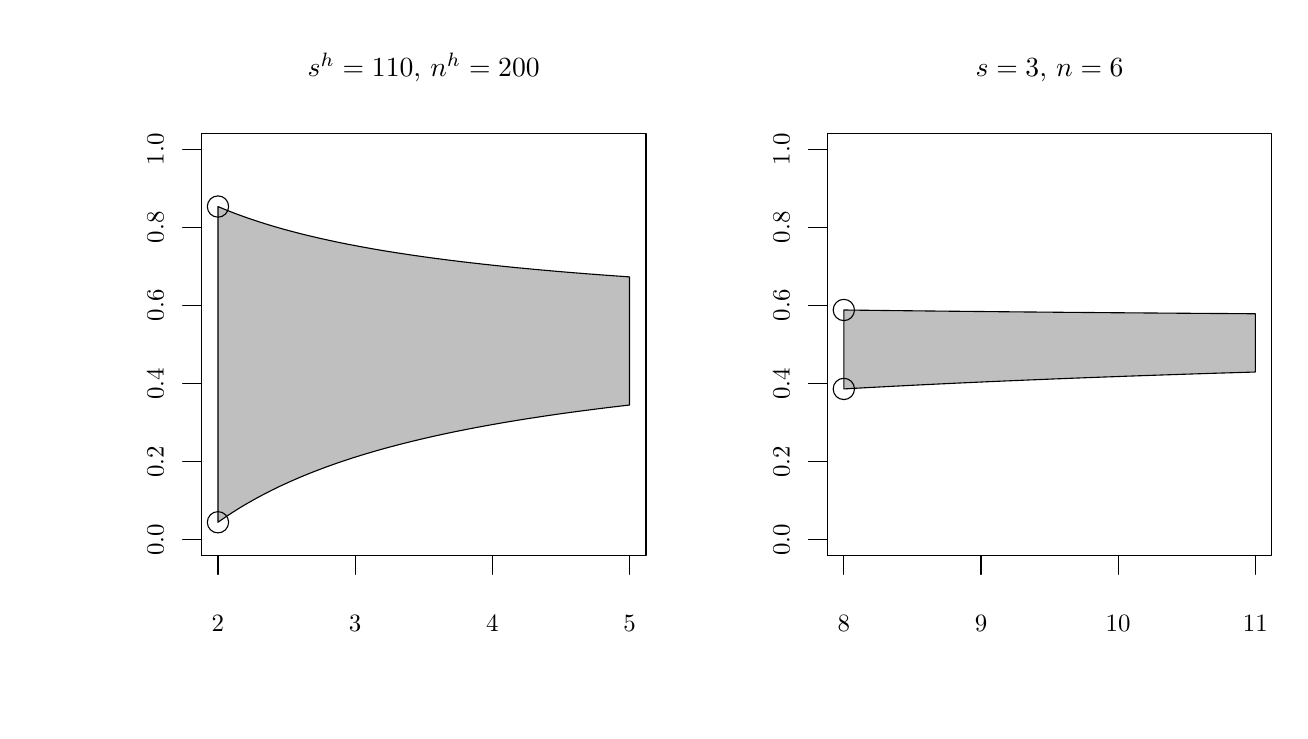
\begin{tikzpicture}
%\pgftransformscale{0.475}
\pgftransformscale{0.04}
%\include{simpleEx.tex}
% Created by tikzDevice version 0.5.0 on 2011-02-28 18:37:21
\begin{scope}
\path[clip] (  0.00,  0.00) rectangle (397.48,216.81);
\definecolor[named]{drawColor}{rgb}{0.35,0.67,0.19}
\definecolor[named]{fillColor}{rgb}{0.03,0.18,0.55}
\definecolor[named]{drawColor}{rgb}{0.00,0.00,0.00}

\draw[color=drawColor,line cap=round,line join=round,fill opacity=0.00,] ( 60.43, 49.20) -- (191.11, 49.20);

\draw[color=drawColor,line cap=round,line join=round,fill opacity=0.00,] ( 60.43, 49.20) -- ( 60.43, 43.20);

\draw[color=drawColor,line cap=round,line join=round,fill opacity=0.00,] (103.99, 49.20) -- (103.99, 43.20);

\draw[color=drawColor,line cap=round,line join=round,fill opacity=0.00,] (147.55, 49.20) -- (147.55, 43.20);

\draw[color=drawColor,line cap=round,line join=round,fill opacity=0.00,] (191.11, 49.20) -- (191.11, 43.20);

\node[color=drawColor,anchor=base,inner sep=0pt, outer sep=0pt, scale=  0.90] at ( 60.43, 25.20) {2%
};

\node[color=drawColor,anchor=base,inner sep=0pt, outer sep=0pt, scale=  0.90] at (103.99, 25.20) {3%
};

\node[color=drawColor,anchor=base,inner sep=0pt, outer sep=0pt, scale=  0.90] at (147.55, 25.20) {4%
};

\node[color=drawColor,anchor=base,inner sep=0pt, outer sep=0pt, scale=  0.90] at (191.11, 25.20) {5%
};

\draw[color=drawColor,line cap=round,line join=round,fill opacity=0.00,] ( 55.20, 54.16) -- ( 55.20,178.25);

\draw[color=drawColor,line cap=round,line join=round,fill opacity=0.00,] ( 55.20, 54.16) -- ( 49.20, 54.16);

\draw[color=drawColor,line cap=round,line join=round,fill opacity=0.00,] ( 55.20, 78.98) -- ( 49.20, 78.98);

\draw[color=drawColor,line cap=round,line join=round,fill opacity=0.00,] ( 55.20,103.80) -- ( 49.20,103.80);

\draw[color=drawColor,line cap=round,line join=round,fill opacity=0.00,] ( 55.20,128.61) -- ( 49.20,128.61);

\draw[color=drawColor,line cap=round,line join=round,fill opacity=0.00,] ( 55.20,153.43) -- ( 49.20,153.43);

\draw[color=drawColor,line cap=round,line join=round,fill opacity=0.00,] ( 55.20,178.25) -- ( 49.20,178.25);

\node[rotate= 90.00,color=drawColor,anchor=base,inner sep=0pt, outer sep=0pt, scale=  0.90] at ( 43.20, 54.16) {0.0%
};

\node[rotate= 90.00,color=drawColor,anchor=base,inner sep=0pt, outer sep=0pt, scale=  0.90] at ( 43.20, 78.98) {0.2%
};

\node[rotate= 90.00,color=drawColor,anchor=base,inner sep=0pt, outer sep=0pt, scale=  0.90] at ( 43.20,103.80) {0.4%
};

\node[rotate= 90.00,color=drawColor,anchor=base,inner sep=0pt, outer sep=0pt, scale=  0.90] at ( 43.20,128.61) {0.6%
};

\node[rotate= 90.00,color=drawColor,anchor=base,inner sep=0pt, outer sep=0pt, scale=  0.90] at ( 43.20,153.43) {0.8%
};

\node[rotate= 90.00,color=drawColor,anchor=base,inner sep=0pt, outer sep=0pt, scale=  0.90] at ( 43.20,178.25) {1.0%
};

\draw[color=drawColor,line cap=round,line join=round,fill opacity=0.00,] ( 55.20, 49.20) --
	(196.34, 49.20) --
	(196.34,183.21) --
	( 55.20,183.21) --
	( 55.20, 49.20);
\end{scope}
\begin{scope}
\path[clip] (  0.00,  0.00) rectangle (198.74,216.81);
\definecolor[named]{drawColor}{rgb}{0.35,0.67,0.19}
\definecolor[named]{fillColor}{rgb}{0.03,0.18,0.55}
\definecolor[named]{drawColor}{rgb}{0.00,0.00,0.00}

\node[color=drawColor,anchor=base,inner sep=0pt, outer sep=0pt, scale=  1.00] at (125.77,  1.20) {$\nz$%
};

\node[rotate= 90.00,color=drawColor,anchor=base,inner sep=0pt, outer sep=0pt, scale=  1.00] at ( 19.20,116.21) {$\yz$%
};
\end{scope}
\begin{scope}
\path[clip] ( 55.20, 49.20) rectangle (196.34,183.21);
\definecolor[named]{drawColor}{rgb}{0.35,0.67,0.19}
\definecolor[named]{fillColor}{rgb}{0.03,0.18,0.55}
\definecolor[named]{drawColor}{rgb}{0.00,0.00,0.00}
\definecolor[named]{fillColor}{rgb}{0.75,0.75,0.75}

\draw[color=drawColor,line cap=round,line join=round,fill=fillColor,] ( 60.43, 59.75) --
	( 61.75, 60.67) --
	( 63.07, 61.57) --
	( 64.39, 62.44) --
	( 65.71, 63.29) --
	( 67.03, 64.12) --
	( 68.35, 64.92) --
	( 69.67, 65.70) --
	( 70.99, 66.45) --
	( 72.31, 67.19) --
	( 73.63, 67.91) --
	( 74.95, 68.61) --
	( 76.27, 69.29) --
	( 77.59, 69.96) --
	( 78.91, 70.60) --
	( 80.23, 71.24) --
	( 81.55, 71.85) --
	( 82.87, 72.45) --
	( 84.19, 73.04) --
	( 85.51, 73.62) --
	( 86.83, 74.18) --
	( 88.15, 74.72) --
	( 89.47, 75.26) --
	( 90.79, 75.78) --
	( 92.11, 76.29) --
	( 93.43, 76.79) --
	( 94.75, 77.28) --
	( 96.07, 77.76) --
	( 97.39, 78.23) --
	( 98.71, 78.69) --
	(100.03, 79.14) --
	(101.35, 79.57) --
	(102.67, 80.01) --
	(103.99, 80.43) --
	(105.31, 80.84) --
	(106.63, 81.25) --
	(107.95, 81.64) --
	(109.27, 82.03) --
	(110.59, 82.42) --
	(111.91, 82.79) --
	(113.23, 83.16) --
	(114.55, 83.52) --
	(115.87, 83.87) --
	(117.19, 84.22) --
	(118.51, 84.56) --
	(119.83, 84.90) --
	(121.15, 85.23) --
	(122.47, 85.55) --
	(123.79, 85.87) --
	(125.11, 86.18) --
	(126.43, 86.49) --
	(127.75, 86.79) --
	(129.07, 87.09) --
	(130.39, 87.38) --
	(131.71, 87.67) --
	(133.03, 87.95) --
	(134.35, 88.23) --
	(135.67, 88.50) --
	(136.99, 88.77) --
	(138.31, 89.03) --
	(139.63, 89.29) --
	(140.95, 89.55) --
	(142.27, 89.80) --
	(143.59, 90.05) --
	(144.91, 90.29) --
	(146.23, 90.53) --
	(147.55, 90.77) --
	(148.87, 91.00) --
	(150.19, 91.23) --
	(151.51, 91.46) --
	(152.83, 91.68) --
	(154.15, 91.90) --
	(155.47, 92.12) --
	(156.79, 92.33) --
	(158.11, 92.54) --
	(159.43, 92.75) --
	(160.75, 92.95) --
	(162.07, 93.15) --
	(163.39, 93.35) --
	(164.71, 93.55) --
	(166.03, 93.74) --
	(167.35, 93.93) --
	(168.67, 94.12) --
	(169.99, 94.31) --
	(171.31, 94.49) --
	(172.63, 94.67) --
	(173.95, 94.85) --
	(175.27, 95.03) --
	(176.59, 95.20) --
	(177.91, 95.37) --
	(179.23, 95.54) --
	(180.55, 95.71) --
	(181.87, 95.87) --
	(183.19, 96.04) --
	(184.51, 96.20) --
	(185.83, 96.36) --
	(187.15, 96.51) --
	(188.47, 96.67) --
	(189.79, 96.82) --
	(191.11, 96.97) --
	(191.11,137.67) --
	(189.79,137.76) --
	(188.47,137.85) --
	(187.15,137.95) --
	(185.83,138.04) --
	(184.51,138.14) --
	(183.19,138.23) --
	(181.87,138.33) --
	(180.55,138.43) --
	(179.23,138.53) --
	(177.91,138.63) --
	(176.59,138.73) --
	(175.27,138.84) --
	(173.95,138.94) --
	(172.63,139.05) --
	(171.31,139.16) --
	(169.99,139.27) --
	(168.67,139.38) --
	(167.35,139.49) --
	(166.03,139.61) --
	(164.71,139.73) --
	(163.39,139.84) --
	(162.07,139.96) --
	(160.75,140.08) --
	(159.43,140.21) --
	(158.11,140.33) --
	(156.79,140.46) --
	(155.47,140.58) --
	(154.15,140.71) --
	(152.83,140.85) --
	(151.51,140.98) --
	(150.19,141.12) --
	(148.87,141.25) --
	(147.55,141.39) --
	(146.23,141.54) --
	(144.91,141.68) --
	(143.59,141.83) --
	(142.27,141.98) --
	(140.95,142.13) --
	(139.63,142.28) --
	(138.31,142.44) --
	(136.99,142.59) --
	(135.67,142.76) --
	(134.35,142.92) --
	(133.03,143.09) --
	(131.71,143.26) --
	(130.39,143.43) --
	(129.07,143.60) --
	(127.75,143.78) --
	(126.43,143.96) --
	(125.11,144.15) --
	(123.79,144.33) --
	(122.47,144.52) --
	(121.15,144.72) --
	(119.83,144.92) --
	(118.51,145.12) --
	(117.19,145.32) --
	(115.87,145.53) --
	(114.55,145.74) --
	(113.23,145.96) --
	(111.91,146.18) --
	(110.59,146.40) --
	(109.27,146.63) --
	(107.95,146.87) --
	(106.63,147.11) --
	(105.31,147.35) --
	(103.99,147.60) --
	(102.67,147.85) --
	(101.35,148.11) --
	(100.03,148.37) --
	( 98.71,148.64) --
	( 97.39,148.92) --
	( 96.07,149.20) --
	( 94.75,149.49) --
	( 93.43,149.78) --
	( 92.11,150.08) --
	( 90.79,150.39) --
	( 89.47,150.70) --
	( 88.15,151.02) --
	( 86.83,151.35) --
	( 85.51,151.69) --
	( 84.19,152.03) --
	( 82.87,152.38) --
	( 81.55,152.74) --
	( 80.23,153.11) --
	( 78.91,153.49) --
	( 77.59,153.88) --
	( 76.27,154.28) --
	( 74.95,154.69) --
	( 73.63,155.11) --
	( 72.31,155.54) --
	( 70.99,155.98) --
	( 69.67,156.44) --
	( 68.35,156.90) --
	( 67.03,157.38) --
	( 65.71,157.88) --
	( 64.39,158.39) --
	( 63.07,158.91) --
	( 61.75,159.45) --
	( 60.43,160.01) --
	cycle;

\draw[color=drawColor,line cap=round,line join=round,fill opacity=0.00,] ( 60.43, 59.75) circle (  3.38);

\draw[color=drawColor,line cap=round,line join=round,fill opacity=0.00,] ( 60.43,160.01) circle (  3.38);
\end{scope}
\begin{scope}
\path[clip] (  0.00,  0.00) rectangle (397.48,216.81);
\definecolor[named]{drawColor}{rgb}{0.35,0.67,0.19}
\definecolor[named]{fillColor}{rgb}{0.03,0.18,0.55}
\definecolor[named]{drawColor}{rgb}{0.00,0.00,0.00}

\node[color=drawColor,anchor=base,inner sep=0pt, outer sep=0pt, scale=  1.00] at (125.77,201.21) {$s^h =  110 $, $n^h =  200 $%
};
\end{scope}
\begin{scope}
\path[clip] (253.94, 49.20) rectangle (395.08,183.21);
\definecolor[named]{drawColor}{rgb}{0.35,0.67,0.19}
\definecolor[named]{fillColor}{rgb}{0.03,0.18,0.55}
\end{scope}
\begin{scope}
\path[clip] (  0.00,  0.00) rectangle (397.48,216.81);
\definecolor[named]{drawColor}{rgb}{0.35,0.67,0.19}
\definecolor[named]{fillColor}{rgb}{0.03,0.18,0.55}
\definecolor[named]{drawColor}{rgb}{0.00,0.00,0.00}

\draw[color=drawColor,line cap=round,line join=round,fill opacity=0.00,] (259.17, 49.20) -- (389.86, 49.20);

\draw[color=drawColor,line cap=round,line join=round,fill opacity=0.00,] (259.17, 49.20) -- (259.17, 43.20);

\draw[color=drawColor,line cap=round,line join=round,fill opacity=0.00,] (302.73, 49.20) -- (302.73, 43.20);

\draw[color=drawColor,line cap=round,line join=round,fill opacity=0.00,] (346.29, 49.20) -- (346.29, 43.20);

\draw[color=drawColor,line cap=round,line join=round,fill opacity=0.00,] (389.86, 49.20) -- (389.86, 43.20);

\node[color=drawColor,anchor=base,inner sep=0pt, outer sep=0pt, scale=  0.90] at (259.17, 25.20) {8%
};

\node[color=drawColor,anchor=base,inner sep=0pt, outer sep=0pt, scale=  0.90] at (302.73, 25.20) {9%
};

\node[color=drawColor,anchor=base,inner sep=0pt, outer sep=0pt, scale=  0.90] at (346.29, 25.20) {10%
};

\node[color=drawColor,anchor=base,inner sep=0pt, outer sep=0pt, scale=  0.90] at (389.86, 25.20) {11%
};

\draw[color=drawColor,line cap=round,line join=round,fill opacity=0.00,] (253.94, 54.16) -- (253.94,178.25);

\draw[color=drawColor,line cap=round,line join=round,fill opacity=0.00,] (253.94, 54.16) -- (247.94, 54.16);

\draw[color=drawColor,line cap=round,line join=round,fill opacity=0.00,] (253.94, 78.98) -- (247.94, 78.98);

\draw[color=drawColor,line cap=round,line join=round,fill opacity=0.00,] (253.94,103.80) -- (247.94,103.80);

\draw[color=drawColor,line cap=round,line join=round,fill opacity=0.00,] (253.94,128.61) -- (247.94,128.61);

\draw[color=drawColor,line cap=round,line join=round,fill opacity=0.00,] (253.94,153.43) -- (247.94,153.43);

\draw[color=drawColor,line cap=round,line join=round,fill opacity=0.00,] (253.94,178.25) -- (247.94,178.25);

\node[rotate= 90.00,color=drawColor,anchor=base,inner sep=0pt, outer sep=0pt, scale=  0.90] at (241.94, 54.16) {0.0%
};

\node[rotate= 90.00,color=drawColor,anchor=base,inner sep=0pt, outer sep=0pt, scale=  0.90] at (241.94, 78.98) {0.2%
};

\node[rotate= 90.00,color=drawColor,anchor=base,inner sep=0pt, outer sep=0pt, scale=  0.90] at (241.94,103.80) {0.4%
};

\node[rotate= 90.00,color=drawColor,anchor=base,inner sep=0pt, outer sep=0pt, scale=  0.90] at (241.94,128.61) {0.6%
};

\node[rotate= 90.00,color=drawColor,anchor=base,inner sep=0pt, outer sep=0pt, scale=  0.90] at (241.94,153.43) {0.8%
};

\node[rotate= 90.00,color=drawColor,anchor=base,inner sep=0pt, outer sep=0pt, scale=  0.90] at (241.94,178.25) {1.0%
};

\draw[color=drawColor,line cap=round,line join=round,fill opacity=0.00,] (253.94, 49.20) --
	(395.08, 49.20) --
	(395.08,183.21) --
	(253.94,183.21) --
	(253.94, 49.20);
\end{scope}
\begin{scope}
\path[clip] (198.74,  0.00) rectangle (397.48,216.81);
\definecolor[named]{drawColor}{rgb}{0.35,0.67,0.19}
\definecolor[named]{fillColor}{rgb}{0.03,0.18,0.55}
\definecolor[named]{drawColor}{rgb}{0.00,0.00,0.00}

\node[color=drawColor,anchor=base,inner sep=0pt, outer sep=0pt, scale=  1.00] at (324.51,  1.20) {$\nn$%
};

\node[rotate= 90.00,color=drawColor,anchor=base,inner sep=0pt, outer sep=0pt, scale=  1.00] at (217.94,116.21) {$\yn$%
};
\end{scope}
\begin{scope}
\path[clip] (253.94, 49.20) rectangle (395.08,183.21);
\definecolor[named]{drawColor}{rgb}{0.35,0.67,0.19}
\definecolor[named]{fillColor}{rgb}{0.03,0.18,0.55}
\definecolor[named]{drawColor}{rgb}{0.00,0.00,0.00}
\definecolor[named]{fillColor}{rgb}{0.75,0.75,0.75}

\draw[color=drawColor,line cap=round,line join=round,fill=fillColor,] (259.17,102.09) --
	(260.49,102.16) --
	(261.81,102.24) --
	(263.13,102.31) --
	(264.45,102.38) --
	(265.77,102.46) --
	(267.09,102.53) --
	(268.41,102.60) --
	(269.73,102.67) --
	(271.05,102.74) --
	(272.37,102.81) --
	(273.69,102.88) --
	(275.01,102.95) --
	(276.33,103.01) --
	(277.65,103.08) --
	(278.97,103.15) --
	(280.29,103.22) --
	(281.61,103.28) --
	(282.93,103.35) --
	(284.25,103.41) --
	(285.57,103.48) --
	(286.89,103.54) --
	(288.21,103.61) --
	(289.53,103.67) --
	(290.85,103.73) --
	(292.17,103.79) --
	(293.49,103.86) --
	(294.81,103.92) --
	(296.13,103.98) --
	(297.45,104.04) --
	(298.77,104.10) --
	(300.09,104.16) --
	(301.41,104.22) --
	(302.73,104.28) --
	(304.05,104.34) --
	(305.37,104.40) --
	(306.69,104.45) --
	(308.01,104.51) --
	(309.33,104.57) --
	(310.65,104.63) --
	(311.97,104.68) --
	(313.29,104.74) --
	(314.61,104.79) --
	(315.93,104.85) --
	(317.25,104.90) --
	(318.57,104.96) --
	(319.89,105.01) --
	(321.21,105.07) --
	(322.53,105.12) --
	(323.85,105.17) --
	(325.17,105.23) --
	(326.49,105.28) --
	(327.81,105.33) --
	(329.13,105.38) --
	(330.45,105.44) --
	(331.77,105.49) --
	(333.09,105.54) --
	(334.41,105.59) --
	(335.73,105.64) --
	(337.05,105.69) --
	(338.37,105.74) --
	(339.69,105.79) --
	(341.01,105.84) --
	(342.33,105.89) --
	(343.65,105.93) --
	(344.97,105.98) --
	(346.29,106.03) --
	(347.62,106.08) --
	(348.94,106.13) --
	(350.26,106.17) --
	(351.58,106.22) --
	(352.90,106.27) --
	(354.22,106.31) --
	(355.54,106.36) --
	(356.86,106.40) --
	(358.18,106.45) --
	(359.50,106.49) --
	(360.82,106.54) --
	(362.14,106.58) --
	(363.46,106.63) --
	(364.78,106.67) --
	(366.10,106.72) --
	(367.42,106.76) --
	(368.74,106.80) --
	(370.06,106.85) --
	(371.38,106.89) --
	(372.70,106.93) --
	(374.02,106.97) --
	(375.34,107.02) --
	(376.66,107.06) --
	(377.98,107.10) --
	(379.30,107.14) --
	(380.62,107.18) --
	(381.94,107.22) --
	(383.26,107.26) --
	(384.58,107.30) --
	(385.90,107.34) --
	(387.22,107.38) --
	(388.54,107.42) --
	(389.86,107.46) --
	(389.86,125.96) --
	(388.54,125.97) --
	(387.22,125.98) --
	(385.90,125.99) --
	(384.58,126.00) --
	(383.26,126.01) --
	(381.94,126.02) --
	(380.62,126.03) --
	(379.30,126.03) --
	(377.98,126.04) --
	(376.66,126.05) --
	(375.34,126.06) --
	(374.02,126.07) --
	(372.70,126.08) --
	(371.38,126.09) --
	(370.06,126.10) --
	(368.74,126.11) --
	(367.42,126.12) --
	(366.10,126.13) --
	(364.78,126.14) --
	(363.46,126.15) --
	(362.14,126.16) --
	(360.82,126.17) --
	(359.50,126.18) --
	(358.18,126.19) --
	(356.86,126.20) --
	(355.54,126.21) --
	(354.22,126.22) --
	(352.90,126.23) --
	(351.58,126.24) --
	(350.26,126.25) --
	(348.94,126.26) --
	(347.62,126.27) --
	(346.29,126.28) --
	(344.97,126.29) --
	(343.65,126.30) --
	(342.33,126.31) --
	(341.01,126.32) --
	(339.69,126.33) --
	(338.37,126.35) --
	(337.05,126.36) --
	(335.73,126.37) --
	(334.41,126.38) --
	(333.09,126.39) --
	(331.77,126.40) --
	(330.45,126.41) --
	(329.13,126.42) --
	(327.81,126.44) --
	(326.49,126.45) --
	(325.17,126.46) --
	(323.85,126.47) --
	(322.53,126.48) --
	(321.21,126.49) --
	(319.89,126.51) --
	(318.57,126.52) --
	(317.25,126.53) --
	(315.93,126.54) --
	(314.61,126.56) --
	(313.29,126.57) --
	(311.97,126.58) --
	(310.65,126.59) --
	(309.33,126.60) --
	(308.01,126.62) --
	(306.69,126.63) --
	(305.37,126.64) --
	(304.05,126.66) --
	(302.73,126.67) --
	(301.41,126.68) --
	(300.09,126.70) --
	(298.77,126.71) --
	(297.45,126.72) --
	(296.13,126.74) --
	(294.81,126.75) --
	(293.49,126.76) --
	(292.17,126.78) --
	(290.85,126.79) --
	(289.53,126.80) --
	(288.21,126.82) --
	(286.89,126.83) --
	(285.57,126.85) --
	(284.25,126.86) --
	(282.93,126.88) --
	(281.61,126.89) --
	(280.29,126.91) --
	(278.97,126.92) --
	(277.65,126.94) --
	(276.33,126.95) --
	(275.01,126.97) --
	(273.69,126.98) --
	(272.37,127.00) --
	(271.05,127.01) --
	(269.73,127.03) --
	(268.41,127.04) --
	(267.09,127.06) --
	(265.77,127.07) --
	(264.45,127.09) --
	(263.13,127.11) --
	(261.81,127.12) --
	(260.49,127.14) --
	(259.17,127.16) --
	cycle;

\draw[color=drawColor,line cap=round,line join=round,fill opacity=0.00,] (259.17,102.09) circle (  3.38);

\draw[color=drawColor,line cap=round,line join=round,fill opacity=0.00,] (259.17,127.16) circle (  3.38);
\end{scope}
\begin{scope}
\path[clip] (  0.00,  0.00) rectangle (397.48,216.81);
\definecolor[named]{drawColor}{rgb}{0.35,0.67,0.19}
\definecolor[named]{fillColor}{rgb}{0.03,0.18,0.55}
\definecolor[named]{drawColor}{rgb}{0.00,0.00,0.00}

\node[color=drawColor,anchor=base,inner sep=0pt, outer sep=0pt, scale=  1.00] at (324.51,201.21) {$s =  3 $, $n =  6 $%
};
\end{scope}

%
\end{tikzpicture}
\caption{$\PZ$ and $\PN$ for the \emph{anteater} shape.}
\label{fig:anteater-ex1}
\end{figure}
%
Rewriting \eqref{equ:anteater-y0}, $\PZ$ is now defined by %\vspace*{-1ex}
%\begin{multline*}
\begin{align*}
%\{ (\nz, \yz) \mid \nz &\in [\nzl, \nzu],\,\\
%                   \yz &\in [ \cl - \frac{n^h}{\nz}\Big(\frac{s^h}{n^h} - \cl\Big),
%                              \cu + \frac{n^h}{\nz}(\cu -\frac{s^h}{n^h})  ] \}\,,
%\hspace*{-2ex}%
\PZ &= 
\Big\{ \Big. (\nz, \yz) \,\Big|\, \nz \in [\nzl, \nzu],\, %\\
%\hspace*{3ex}     
                  \yz(\nz) \in \Big[ \cl - \frac{n^h}{\nz}\Big(\frac{s^h}{n^h} - \cl\Big),\,
                                     \cu + \frac{n^h}{\nz}\Big(\cu - \frac{s^h}{n^h}\Big)  \Big] \Big\}\,.
\end{align*}
%\end{multline*}
With the reasonable choice of $\cl$ and $\cu$ such that $\cl \leq s^h/n^h \leq \cu$,
$\PZ$ can be interpreted as follows: The range of $\yz$
protrudes over $[\cl, \cu]$
on either side far enough to ensure $\Pl = \cl$ and $\Pu = \cu$ if
updated with $s = s^h$ for $n = n^h$, the amount of protrusion
decreasing in $\nz$ as the movement of $\yz(\nz)$ towards $s^h/n^h$ is slower
for larger values of $\nz$. As there is a considerable difference in behaviour if
$n > n^h$ or $n < n^h$, these two cases are discussed separately.

If $n > n^h$, the PPP graph in Figure~\ref{fig:priorset-generic}
holds again, now with the values
\begin{align*}
A   &= \frac{\cl (\nzl + n^h) - s^h}    {\nzl + n} & % \frac{\nzl \yzl}{\nzl + n} &
S_1 &= s^h + \cl (n - n^h) \\ % n\yzl &
B   &= \frac{\cu (\nzu + n^h) - s^h}    {\nzu + n} & % \frac{\nzu \yzu}{\nzu + n} \\
S_2 &= s^h + \cu (n - n^h) \\ % n\yzu \\
%\end{align*}%\vspace*{-4ex}
%\begin{align*}
C   &= \frac{\cl (\nzu + n^h) - s^h + n}{\nzu + n} & % \frac{\nzu \yzl + n}{\nzu + n} &
\text{sl.~1} &= 1/(\nzu + n) \\
D   &= \frac{\cu (\nzl + n^h) - s^h + n}{\nzl + n} &  % \frac{\nzl \yzu + n}{\nzl + n} \\
\text{sl.~2} &= 1/(\nzl + n)
%\text{sl.~1} &= \frac{1}{\nzu + n} &
%\text{sl.~2} &= \frac{1}{\nzl + n}
\end{align*}%\vspace*{-4ex}
\begin{align*}
E_1 &= \cl &
E_2 &= \cl + \frac{\nzu + n^h }{\nzu + n} (\cu - \cl) %&
     = \cu - \frac{ n   - n^h }{\nzu + n} (\cu - \cl) \\ % \frac{\nzu \yzu + n \yzl}{\nzu + n} \\
F_2 &= \cu &
F_1 &= \cu - \frac{\nzu + n^h }{\nzu + n} (\cu - \cl) %&
     = \cl + \frac{ n   - n^h }{\nzu + n} (\cu - \cl) \,.% \frac{\nzu \yzl + n \yzu}{\nzu + n} &
\end{align*}
As for the pdc-IBBM, the TPDA boundaries $S_1$ and $S_2$ mark the transition points
where either $\ynl$ or $\ynu$ are constant in $\nz$. We now have
\begin{align*}
\frac{S_1}{n} &= \cl + \frac{n^h}{n}\Big( \frac{s^h}{n^h} - \cl \Big), &
\frac{S_2}{n} &= \cu - \frac{n^h}{n}\Big( \cu - \frac{s^h}{n^h} \Big),
\end{align*}
so this TPDA is a subset of $[\cl, \cu]$. The \emph{anteater}
shape is, for $n>n^h$, even more strict than the pdc-IBBM, as, e.g.,
$\yzl(\nzu) = \cl - \frac{n^h}{\nzu}\big( \frac{s^h}{n^h} - \cl \big) < \frac{S_1}{n}$.


The situation for $n < n^h$ is illustrated in Figure~\ref{fig:anteater-nsmall},
where $A$, $B$, $C$, $D$, $E_1$, $F_2$ and slopes 1 and 2 are the same as for $n > n^h$, but
\begin{align*}
E_2 &= \cl + \frac{\nzl + n^h }{\nzl + n} (\cu - \cl) %&
     = \cu + \frac{ n^h - n   }{\nzl + n} (\cu - \cl) \,,\\ % \frac{\nzu \yzu + n \yzl}{\nzu + n} \\
F_1 &= \cu - \frac{\nzl + n^h }{\nzl + n} (\cu - \cl) %&
     = \cl - \frac{ n^h - n   }{\nzl + n} (\cu - \cl) \,.%    \frac{\nzu \yzl + n \yzu}{\nzu + n} &
\end{align*}
Note that now $S_2<S_1$, so the TPDA is $[S_2, S_1]$. In this interval, $\Pl$ and $\Pu$ are now
calculated with $\nzl$; for $s \not\in [S_2, S_1]$ the same situation
as for $n > n^h$ applies, with the bound nearer to $s/n$
calculated with $\nzl$ and the other with $\nzu$.

\begin{figure}%[h]
\centering %
\begin{tikzpicture}
\pgftransformscale{0.8}
%\pgftransformscale{0.475}
\draw[thick] (15,10) -- (0,10) node[left] {\small 1} -- (0,0) node[left] {\small 0} node[below] (Zero) {\small 0} -- node[below,pos=0.3] {\tikz\draw[-stealth,thick] (0,0) -- (1,0) node[right] {\small $s$};} (15,0) -- cycle; %node[below] {n}
\node[node distance=11.6, base right=of Zero] {n};
\coordinate (S2) at (8,0);
\coordinate (S1) at (10,0);
\foreach \point/\name in {S1/S_1, S2/S_2}
 \draw[dashed] (\point) node[below] {\small $\name$} -- ++(0,10);
\coordinate (A) at (0,0.5);
\coordinate (El) at ($(S1) + (0,5.5)$);
\coordinate (C) at ($(El) + (5,1)$);
\coordinate (Fl) at ($(A)!{8/10}!(El)$);
%
\coordinate (D) at (15,9.5);
\coordinate (Fu) at ($(S2) + (0,6)$);
\coordinate (B) at ($(Fu) + (-8,-8/5)$);
\coordinate (Eu) at ($(Fu)!{2/7}!(D)$);
%
\draw[fill] (A) node[above left=-3pt and 0pt] {\small $A$} circle (2pt) ;
\draw[fill] (B) node[left] {\small $B$} circle (2pt) ;
\foreach \point in {C, D}
 \draw[fill] (\point) node[right] {\small $\point$} circle (2pt) ;
\foreach \point/\name in {El/E_1, Eu/E_2}
 \draw[fill] (\point) node[below right=-3pt and -2pt] {\small $\name$} circle (2pt) ;
\foreach \point/\name in {Fl/F_1, Fu/F_2}
 \draw[fill] (\point) node[above  left=-3pt and -2pt] {\small $\name$} circle (2pt) ;
\draw (B) -- node[sloped,below] {\small sl.~1} (Fu) -- node[sloped,above,pos=0.55] {\small sl.~2} (Eu) -- node[sloped,above] {\small sl.~2} (D);
\draw (A) -- node[sloped,below] {\small sl.~2} (Fl) -- node[sloped,below,pos=0.45] {\small sl.~2} (El) -- node[sloped,above] {\small sl.~1} (C);
\end{tikzpicture}
\caption{%$\Pl$ and $\Pu$
\underline{P}\ and $\Pu$
%Lower and upper predictive probability of success
for the \emph{anteater} shape if $n < n^h$.}
\label{fig:anteater-nsmall}
\end{figure}
%
%

\begin{figure}%[h]
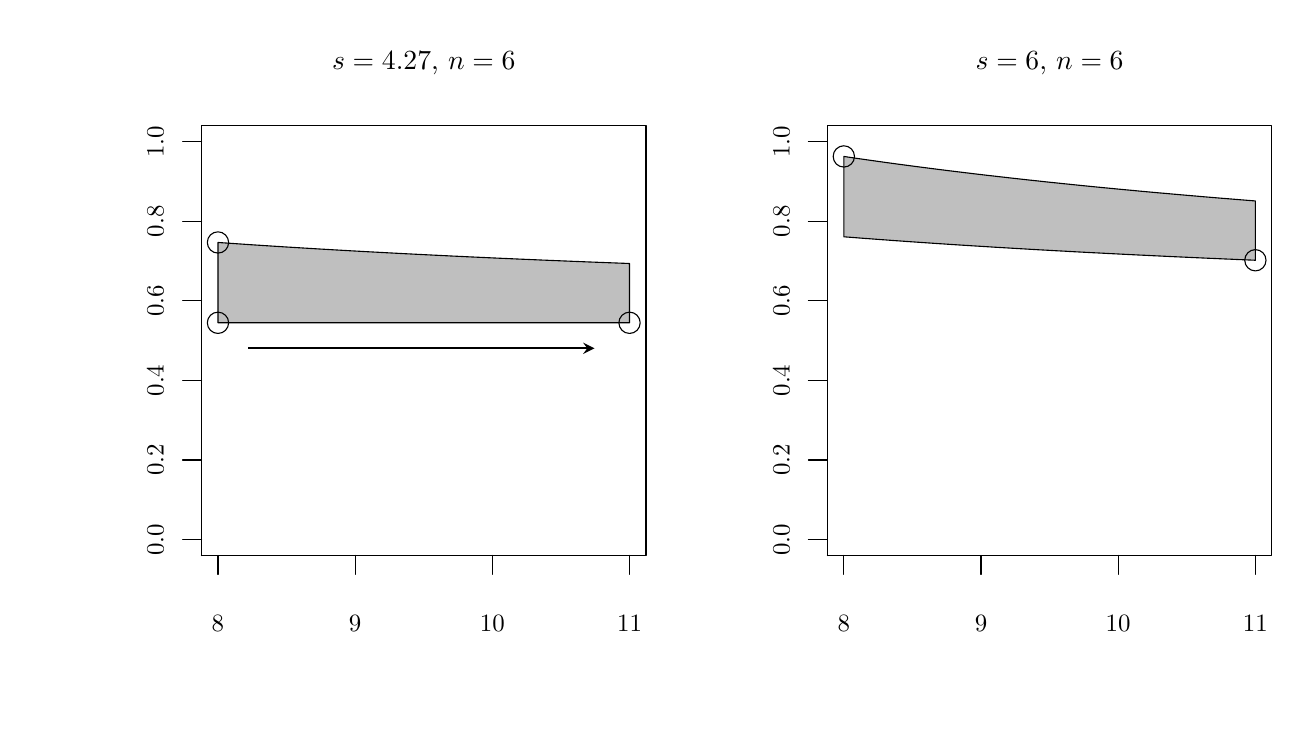
\begin{tikzpicture}
%\pgftransformscale{0.475}
\pgftransformscale{0.04}
%\include{simpleEx.tex}
% Created by tikzDevice version 0.5.0 on 2011-02-28 18:40:33
\begin{scope}
\path[clip] (  0.00,  0.00) rectangle (397.48,216.81);
\definecolor[named]{drawColor}{rgb}{0.03,0.18,0.55}
\definecolor[named]{fillColor}{rgb}{0.88,0.08,0.52}
\definecolor[named]{drawColor}{rgb}{0.00,0.00,0.00}

\draw[color=drawColor,line cap=round,line join=round,fill opacity=0.00,] ( 60.43, 49.20) -- (191.12, 49.20);

\draw[color=drawColor,line cap=round,line join=round,fill opacity=0.00,] ( 60.43, 49.20) -- ( 60.43, 43.20);

\draw[color=drawColor,line cap=round,line join=round,fill opacity=0.00,] (103.99, 49.20) -- (103.99, 43.20);

\draw[color=drawColor,line cap=round,line join=round,fill opacity=0.00,] (147.55, 49.20) -- (147.55, 43.20);

\draw[color=drawColor,line cap=round,line join=round,fill opacity=0.00,] (191.12, 49.20) -- (191.12, 43.20);

\node[color=drawColor,anchor=base,inner sep=0pt, outer sep=0pt, scale=  0.90] at ( 60.43, 25.20) {8%
};

\node[color=drawColor,anchor=base,inner sep=0pt, outer sep=0pt, scale=  0.90] at (103.99, 25.20) {9%
};

\node[color=drawColor,anchor=base,inner sep=0pt, outer sep=0pt, scale=  0.90] at (147.55, 25.20) {10%
};

\node[color=drawColor,anchor=base,inner sep=0pt, outer sep=0pt, scale=  0.90] at (191.12, 25.20) {11%
};

\draw[color=drawColor,line cap=round,line join=round,fill opacity=0.00,] ( 55.20, 54.25) -- ( 55.20,180.56);

\draw[color=drawColor,line cap=round,line join=round,fill opacity=0.00,] ( 55.20, 54.25) -- ( 49.20, 54.25);

\draw[color=drawColor,line cap=round,line join=round,fill opacity=0.00,] ( 55.20, 79.51) -- ( 49.20, 79.51);

\draw[color=drawColor,line cap=round,line join=round,fill opacity=0.00,] ( 55.20,104.77) -- ( 49.20,104.77);

\draw[color=drawColor,line cap=round,line join=round,fill opacity=0.00,] ( 55.20,130.04) -- ( 49.20,130.04);

\draw[color=drawColor,line cap=round,line join=round,fill opacity=0.00,] ( 55.20,155.30) -- ( 49.20,155.30);

\draw[color=drawColor,line cap=round,line join=round,fill opacity=0.00,] ( 55.20,180.56) -- ( 49.20,180.56);

\node[rotate= 90.00,color=drawColor,anchor=base,inner sep=0pt, outer sep=0pt, scale=  0.90] at ( 43.20, 54.25) {0.0%
};

\node[rotate= 90.00,color=drawColor,anchor=base,inner sep=0pt, outer sep=0pt, scale=  0.90] at ( 43.20, 79.51) {0.2%
};

\node[rotate= 90.00,color=drawColor,anchor=base,inner sep=0pt, outer sep=0pt, scale=  0.90] at ( 43.20,104.77) {0.4%
};

\node[rotate= 90.00,color=drawColor,anchor=base,inner sep=0pt, outer sep=0pt, scale=  0.90] at ( 43.20,130.04) {0.6%
};

\node[rotate= 90.00,color=drawColor,anchor=base,inner sep=0pt, outer sep=0pt, scale=  0.90] at ( 43.20,155.30) {0.8%
};

\node[rotate= 90.00,color=drawColor,anchor=base,inner sep=0pt, outer sep=0pt, scale=  0.90] at ( 43.20,180.56) {1.0%
};

\draw[color=drawColor,line cap=round,line join=round,fill opacity=0.00,] ( 55.20, 49.20) --
	(196.34, 49.20) --
	(196.34,185.61) --
	( 55.20,185.61) --
	( 55.20, 49.20);
\end{scope}
\begin{scope}
\path[clip] (  0.00,  0.00) rectangle (198.74,216.81);
\definecolor[named]{drawColor}{rgb}{0.03,0.18,0.55}
\definecolor[named]{fillColor}{rgb}{0.88,0.08,0.52}
\definecolor[named]{drawColor}{rgb}{0.00,0.00,0.00}

\node[color=drawColor,anchor=base,inner sep=0pt, outer sep=0pt, scale=  1.00] at (125.77,  1.20) {$\nn$%
};

\node[rotate= 90.00,color=drawColor,anchor=base,inner sep=0pt, outer sep=0pt, scale=  1.00] at ( 19.20,117.41) {$\yn$%
};
\end{scope}
\begin{scope}
\path[clip] ( 55.20, 49.20) rectangle (196.34,185.61);
\definecolor[named]{drawColor}{rgb}{0.03,0.18,0.55}
\definecolor[named]{fillColor}{rgb}{0.88,0.08,0.52}
\definecolor[named]{drawColor}{rgb}{0.00,0.00,0.00}
\definecolor[named]{fillColor}{rgb}{0.75,0.75,0.75}

\draw[color=drawColor,line cap=round,line join=round,fill=fillColor,] ( 60.43,123.09) --
	( 61.75,123.09) --
	( 63.07,123.09) --
	( 64.39,123.09) --
	( 65.71,123.09) --
	( 67.03,123.09) --
	( 68.35,123.09) --
	( 69.67,123.09) --
	( 70.99,123.09) --
	( 72.31,123.09) --
	( 73.63,123.09) --
	( 74.95,123.09) --
	( 76.27,123.09) --
	( 77.59,123.09) --
	( 78.91,123.09) --
	( 80.23,123.09) --
	( 81.55,123.09) --
	( 82.87,123.09) --
	( 84.19,123.09) --
	( 85.51,123.09) --
	( 86.83,123.09) --
	( 88.15,123.09) --
	( 89.47,123.09) --
	( 90.79,123.09) --
	( 92.11,123.09) --
	( 93.43,123.09) --
	( 94.75,123.09) --
	( 96.07,123.09) --
	( 97.39,123.09) --
	( 98.71,123.09) --
	(100.03,123.09) --
	(101.35,123.09) --
	(102.67,123.09) --
	(103.99,123.09) --
	(105.31,123.09) --
	(106.63,123.09) --
	(107.95,123.09) --
	(109.27,123.09) --
	(110.59,123.09) --
	(111.91,123.09) --
	(113.23,123.09) --
	(114.55,123.09) --
	(115.87,123.09) --
	(117.19,123.09) --
	(118.51,123.09) --
	(119.83,123.09) --
	(121.15,123.09) --
	(122.47,123.09) --
	(123.79,123.09) --
	(125.11,123.09) --
	(126.43,123.09) --
	(127.75,123.09) --
	(129.07,123.09) --
	(130.39,123.09) --
	(131.71,123.09) --
	(133.03,123.09) --
	(134.35,123.09) --
	(135.67,123.09) --
	(136.99,123.09) --
	(138.31,123.09) --
	(139.63,123.09) --
	(140.95,123.09) --
	(142.27,123.09) --
	(143.59,123.09) --
	(144.91,123.09) --
	(146.23,123.09) --
	(147.55,123.09) --
	(148.87,123.09) --
	(150.19,123.09) --
	(151.51,123.09) --
	(152.83,123.09) --
	(154.15,123.09) --
	(155.47,123.09) --
	(156.79,123.09) --
	(158.11,123.09) --
	(159.43,123.09) --
	(160.75,123.09) --
	(162.07,123.09) --
	(163.39,123.09) --
	(164.71,123.09) --
	(166.03,123.09) --
	(167.35,123.09) --
	(168.67,123.09) --
	(169.99,123.09) --
	(171.31,123.09) --
	(172.63,123.09) --
	(173.95,123.09) --
	(175.27,123.09) --
	(176.59,123.09) --
	(177.91,123.09) --
	(179.23,123.09) --
	(180.55,123.09) --
	(181.87,123.09) --
	(183.19,123.09) --
	(184.51,123.09) --
	(185.83,123.09) --
	(187.15,123.09) --
	(188.47,123.09) --
	(189.79,123.09) --
	(191.12,123.09) --
	(191.12,141.92) --
	(189.79,141.97) --
	(188.47,142.02) --
	(187.15,142.07) --
	(185.83,142.12) --
	(184.51,142.17) --
	(183.19,142.22) --
	(181.87,142.27) --
	(180.55,142.32) --
	(179.23,142.37) --
	(177.91,142.42) --
	(176.59,142.48) --
	(175.27,142.53) --
	(173.95,142.58) --
	(172.63,142.63) --
	(171.31,142.69) --
	(169.99,142.74) --
	(168.67,142.80) --
	(167.35,142.85) --
	(166.03,142.90) --
	(164.71,142.96) --
	(163.39,143.01) --
	(162.07,143.07) --
	(160.75,143.13) --
	(159.43,143.18) --
	(158.11,143.24) --
	(156.79,143.29) --
	(155.47,143.35) --
	(154.15,143.41) --
	(152.83,143.47) --
	(151.51,143.53) --
	(150.19,143.58) --
	(148.87,143.64) --
	(147.55,143.70) --
	(146.23,143.76) --
	(144.91,143.82) --
	(143.59,143.88) --
	(142.27,143.94) --
	(140.95,144.00) --
	(139.63,144.06) --
	(138.31,144.13) --
	(136.99,144.19) --
	(135.67,144.25) --
	(134.35,144.31) --
	(133.03,144.38) --
	(131.71,144.44) --
	(130.39,144.51) --
	(129.07,144.57) --
	(127.75,144.64) --
	(126.43,144.70) --
	(125.11,144.77) --
	(123.79,144.83) --
	(122.47,144.90) --
	(121.15,144.97) --
	(119.83,145.03) --
	(118.51,145.10) --
	(117.19,145.17) --
	(115.87,145.24) --
	(114.55,145.31) --
	(113.23,145.38) --
	(111.91,145.45) --
	(110.59,145.52) --
	(109.27,145.59) --
	(107.95,145.66) --
	(106.63,145.73) --
	(105.31,145.81) --
	(103.99,145.88) --
	(102.67,145.95) --
	(101.35,146.03) --
	(100.03,146.10) --
	( 98.71,146.18) --
	( 97.39,146.25) --
	( 96.07,146.33) --
	( 94.75,146.41) --
	( 93.43,146.48) --
	( 92.11,146.56) --
	( 90.79,146.64) --
	( 89.47,146.72) --
	( 88.15,146.80) --
	( 86.83,146.88) --
	( 85.51,146.96) --
	( 84.19,147.04) --
	( 82.87,147.12) --
	( 81.55,147.20) --
	( 80.23,147.29) --
	( 78.91,147.37) --
	( 77.59,147.45) --
	( 76.27,147.54) --
	( 74.95,147.62) --
	( 73.63,147.71) --
	( 72.31,147.79) --
	( 70.99,147.88) --
	( 69.67,147.97) --
	( 68.35,148.06) --
	( 67.03,148.15) --
	( 65.71,148.24) --
	( 64.39,148.33) --
	( 63.07,148.42) --
	( 61.75,148.51) --
	( 60.43,148.60) --
	cycle;

\draw[color=drawColor,line cap=round,line join=round,fill opacity=0.00,] ( 60.43,123.09) circle (  3.38);

\draw[color=drawColor,line cap=round,line join=round,fill opacity=0.00,] (191.12,123.09) circle (  3.38);

\draw[color=drawColor,line cap=round,line join=round,fill opacity=0.00,] ( 60.43,148.60) circle (  3.38);
\end{scope}
\begin{scope}
\path[clip] (  0.00,  0.00) rectangle (397.48,216.81);
\definecolor[named]{drawColor}{rgb}{0.03,0.18,0.55}
\definecolor[named]{fillColor}{rgb}{0.88,0.08,0.52}
\definecolor[named]{drawColor}{rgb}{0.00,0.00,0.00}

\node[color=drawColor,anchor=base,inner sep=0pt, outer sep=0pt, scale=  1.00] at (125.77,203.61) {$s =  4.27 $, $n =  6 $%
};
\end{scope}
\begin{scope}
\path[clip] (253.94, 49.20) rectangle (395.08,185.61);
\definecolor[named]{drawColor}{rgb}{0.03,0.18,0.55}
\definecolor[named]{fillColor}{rgb}{0.88,0.08,0.52}
\end{scope}
\begin{scope}
\path[clip] (  0.00,  0.00) rectangle (397.48,216.81);
\definecolor[named]{drawColor}{rgb}{0.03,0.18,0.55}
\definecolor[named]{fillColor}{rgb}{0.88,0.08,0.52}
\definecolor[named]{drawColor}{rgb}{0.00,0.00,0.00}

\draw[color=drawColor,line cap=round,line join=round,fill opacity=0.00,] (259.17, 49.20) -- (389.86, 49.20);

\draw[color=drawColor,line cap=round,line join=round,fill opacity=0.00,] (259.17, 49.20) -- (259.17, 43.20);

\draw[color=drawColor,line cap=round,line join=round,fill opacity=0.00,] (302.73, 49.20) -- (302.73, 43.20);

\draw[color=drawColor,line cap=round,line join=round,fill opacity=0.00,] (346.29, 49.20) -- (346.29, 43.20);

\draw[color=drawColor,line cap=round,line join=round,fill opacity=0.00,] (389.86, 49.20) -- (389.86, 43.20);

\node[color=drawColor,anchor=base,inner sep=0pt, outer sep=0pt, scale=  0.90] at (259.17, 25.20) {8%
};

\node[color=drawColor,anchor=base,inner sep=0pt, outer sep=0pt, scale=  0.90] at (302.73, 25.20) {9%
};

\node[color=drawColor,anchor=base,inner sep=0pt, outer sep=0pt, scale=  0.90] at (346.29, 25.20) {10%
};

\node[color=drawColor,anchor=base,inner sep=0pt, outer sep=0pt, scale=  0.90] at (389.86, 25.20) {11%
};

\draw[color=drawColor,line cap=round,line join=round,fill opacity=0.00,] (253.94, 54.25) -- (253.94,180.56);

\draw[color=drawColor,line cap=round,line join=round,fill opacity=0.00,] (253.94, 54.25) -- (247.94, 54.25);

\draw[color=drawColor,line cap=round,line join=round,fill opacity=0.00,] (253.94, 79.51) -- (247.94, 79.51);

\draw[color=drawColor,line cap=round,line join=round,fill opacity=0.00,] (253.94,104.77) -- (247.94,104.77);

\draw[color=drawColor,line cap=round,line join=round,fill opacity=0.00,] (253.94,130.04) -- (247.94,130.04);

\draw[color=drawColor,line cap=round,line join=round,fill opacity=0.00,] (253.94,155.30) -- (247.94,155.30);

\draw[color=drawColor,line cap=round,line join=round,fill opacity=0.00,] (253.94,180.56) -- (247.94,180.56);

\node[rotate= 90.00,color=drawColor,anchor=base,inner sep=0pt, outer sep=0pt, scale=  0.90] at (241.94, 54.25) {0.0%
};

\node[rotate= 90.00,color=drawColor,anchor=base,inner sep=0pt, outer sep=0pt, scale=  0.90] at (241.94, 79.51) {0.2%
};

\node[rotate= 90.00,color=drawColor,anchor=base,inner sep=0pt, outer sep=0pt, scale=  0.90] at (241.94,104.77) {0.4%
};

\node[rotate= 90.00,color=drawColor,anchor=base,inner sep=0pt, outer sep=0pt, scale=  0.90] at (241.94,130.04) {0.6%
};

\node[rotate= 90.00,color=drawColor,anchor=base,inner sep=0pt, outer sep=0pt, scale=  0.90] at (241.94,155.30) {0.8%
};

\node[rotate= 90.00,color=drawColor,anchor=base,inner sep=0pt, outer sep=0pt, scale=  0.90] at (241.94,180.56) {1.0%
};

\draw[color=drawColor,line cap=round,line join=round,fill opacity=0.00,] (253.94, 49.20) --
	(395.08, 49.20) --
	(395.08,185.61) --
	(253.94,185.61) --
	(253.94, 49.20);
\end{scope}
\begin{scope}
\path[clip] (198.74,  0.00) rectangle (397.48,216.81);
\definecolor[named]{drawColor}{rgb}{0.03,0.18,0.55}
\definecolor[named]{fillColor}{rgb}{0.88,0.08,0.52}
\definecolor[named]{drawColor}{rgb}{0.00,0.00,0.00}

\node[color=drawColor,anchor=base,inner sep=0pt, outer sep=0pt, scale=  1.00] at (324.51,  1.20) {$\nn$%
};

\node[rotate= 90.00,color=drawColor,anchor=base,inner sep=0pt, outer sep=0pt, scale=  1.00] at (217.94,117.41) {$\yn$%
};
\end{scope}
\begin{scope}
\path[clip] (253.94, 49.20) rectangle (395.08,185.61);
\definecolor[named]{drawColor}{rgb}{0.03,0.18,0.55}
\definecolor[named]{fillColor}{rgb}{0.88,0.08,0.52}
\definecolor[named]{drawColor}{rgb}{0.00,0.00,0.00}
\definecolor[named]{fillColor}{rgb}{0.75,0.75,0.75}

\draw[color=drawColor,line cap=round,line join=round,fill=fillColor,] (259.17,150.40) --
	(260.49,150.30) --
	(261.81,150.20) --
	(263.13,150.10) --
	(264.45,149.99) --
	(265.77,149.89) --
	(267.09,149.80) --
	(268.41,149.70) --
	(269.73,149.60) --
	(271.05,149.50) --
	(272.37,149.41) --
	(273.69,149.31) --
	(275.01,149.21) --
	(276.33,149.12) --
	(277.65,149.03) --
	(278.97,148.93) --
	(280.29,148.84) --
	(281.61,148.75) --
	(282.93,148.66) --
	(284.25,148.57) --
	(285.57,148.48) --
	(286.89,148.39) --
	(288.21,148.30) --
	(289.53,148.21) --
	(290.85,148.13) --
	(292.17,148.04) --
	(293.49,147.95) --
	(294.81,147.87) --
	(296.13,147.78) --
	(297.45,147.70) --
	(298.77,147.62) --
	(300.09,147.53) --
	(301.41,147.45) --
	(302.73,147.37) --
	(304.05,147.29) --
	(305.37,147.21) --
	(306.69,147.12) --
	(308.01,147.04) --
	(309.33,146.97) --
	(310.65,146.89) --
	(311.97,146.81) --
	(313.29,146.73) --
	(314.61,146.65) --
	(315.93,146.58) --
	(317.25,146.50) --
	(318.57,146.42) --
	(319.89,146.35) --
	(321.21,146.27) --
	(322.53,146.20) --
	(323.85,146.13) --
	(325.17,146.05) --
	(326.49,145.98) --
	(327.81,145.91) --
	(329.13,145.84) --
	(330.45,145.76) --
	(331.77,145.69) --
	(333.09,145.62) --
	(334.41,145.55) --
	(335.73,145.48) --
	(337.05,145.41) --
	(338.37,145.34) --
	(339.69,145.28) --
	(341.01,145.21) --
	(342.33,145.14) --
	(343.65,145.07) --
	(344.97,145.01) --
	(346.29,144.94) --
	(347.62,144.87) --
	(348.94,144.81) --
	(350.26,144.74) --
	(351.58,144.68) --
	(352.90,144.61) --
	(354.22,144.55) --
	(355.54,144.49) --
	(356.86,144.42) --
	(358.18,144.36) --
	(359.50,144.30) --
	(360.82,144.23) --
	(362.14,144.17) --
	(363.46,144.11) --
	(364.78,144.05) --
	(366.10,143.99) --
	(367.42,143.93) --
	(368.74,143.87) --
	(370.06,143.81) --
	(371.38,143.75) --
	(372.70,143.69) --
	(374.02,143.63) --
	(375.34,143.57) --
	(376.66,143.52) --
	(377.98,143.46) --
	(379.30,143.40) --
	(380.62,143.34) --
	(381.94,143.29) --
	(383.26,143.23) --
	(384.58,143.17) --
	(385.90,143.12) --
	(387.22,143.06) --
	(388.54,143.01) --
	(389.86,142.95) --
	(389.86,161.78) --
	(388.54,161.89) --
	(387.22,161.99) --
	(385.90,162.10) --
	(384.58,162.20) --
	(383.26,162.31) --
	(381.94,162.42) --
	(380.62,162.53) --
	(379.30,162.63) --
	(377.98,162.74) --
	(376.66,162.85) --
	(375.34,162.96) --
	(374.02,163.07) --
	(372.70,163.18) --
	(371.38,163.30) --
	(370.06,163.41) --
	(368.74,163.52) --
	(367.42,163.64) --
	(366.10,163.75) --
	(364.78,163.87) --
	(363.46,163.98) --
	(362.14,164.10) --
	(360.82,164.22) --
	(359.50,164.33) --
	(358.18,164.45) --
	(356.86,164.57) --
	(355.54,164.69) --
	(354.22,164.81) --
	(352.90,164.93) --
	(351.58,165.06) --
	(350.26,165.18) --
	(348.94,165.30) --
	(347.62,165.43) --
	(346.29,165.55) --
	(344.97,165.68) --
	(343.65,165.81) --
	(342.33,165.93) --
	(341.01,166.06) --
	(339.69,166.19) --
	(338.37,166.32) --
	(337.05,166.45) --
	(335.73,166.58) --
	(334.41,166.71) --
	(333.09,166.85) --
	(331.77,166.98) --
	(330.45,167.12) --
	(329.13,167.25) --
	(327.81,167.39) --
	(326.49,167.53) --
	(325.17,167.66) --
	(323.85,167.80) --
	(322.53,167.94) --
	(321.21,168.09) --
	(319.89,168.23) --
	(318.57,168.37) --
	(317.25,168.51) --
	(315.93,168.66) --
	(314.61,168.80) --
	(313.29,168.95) --
	(311.97,169.10) --
	(310.65,169.25) --
	(309.33,169.40) --
	(308.01,169.55) --
	(306.69,169.70) --
	(305.37,169.85) --
	(304.05,170.00) --
	(302.73,170.16) --
	(301.41,170.31) --
	(300.09,170.47) --
	(298.77,170.63) --
	(297.45,170.79) --
	(296.13,170.95) --
	(294.81,171.11) --
	(293.49,171.27) --
	(292.17,171.43) --
	(290.85,171.60) --
	(289.53,171.76) --
	(288.21,171.93) --
	(286.89,172.10) --
	(285.57,172.27) --
	(284.25,172.44) --
	(282.93,172.61) --
	(281.61,172.78) --
	(280.29,172.96) --
	(278.97,173.13) --
	(277.65,173.31) --
	(276.33,173.48) --
	(275.01,173.66) --
	(273.69,173.84) --
	(272.37,174.02) --
	(271.05,174.21) --
	(269.73,174.39) --
	(268.41,174.58) --
	(267.09,174.76) --
	(265.77,174.95) --
	(264.45,175.14) --
	(263.13,175.33) --
	(261.81,175.53) --
	(260.49,175.72) --
	(259.17,175.92) --
	cycle;

\draw[color=drawColor,line cap=round,line join=round,fill opacity=0.00,] (389.86,142.95) circle (  3.38);

\draw[color=drawColor,line cap=round,line join=round,fill opacity=0.00,] (259.17,175.92) circle (  3.38);
\end{scope}
\begin{scope}
\path[clip] (  0.00,  0.00) rectangle (397.48,216.81);
\definecolor[named]{drawColor}{rgb}{0.03,0.18,0.55}
\definecolor[named]{fillColor}{rgb}{0.88,0.08,0.52}
\definecolor[named]{drawColor}{rgb}{0.00,0.00,0.00}

\node[color=drawColor,anchor=base,inner sep=0pt, outer sep=0pt, scale=  1.00] at (324.51,203.61) {$s =  6 $, $n =  6 $%
};
\end{scope}

\draw[-stealth, thick] (70,115) -- (180,115);
%\draw (0,0) rectangle (400, 220);
%
\end{tikzpicture}
\caption[Posterior parameter sets $\PN$ for \emph{anteater} prior sets $\PZ$.]%
{Posterior parameter sets $\PN$ for \emph{anteater} prior sets $\PZ$.
Left: the transition point where %$\ynl$
the lower contour of the posterior parameter set 
is attained for all $\nn$, right: the \emph{banana} shape.}
\label{fig:anteater-ex2}
\end{figure}



%The case of $n < n^h$ seems the most useful,
%Considering the upper switch point $S_1$ (analogue findings hold for $S_2$),
The upper transition point $S_1$ can now be between $\yzu(\nzl)$ and $\yzu(\nzu)$, and having
$S_1$ decreasing in $n$ now makes sense: the smaller $n$, the larger $S_1$, i.e.\
the more tolerant is the \emph{anteater} set.
The switch over $S_1$ (with $s/n$ increasing)
%The switch over the upper transition point $S_1$ (with $s/n$ increasing) \com{in the case of $n < n^h$}
is illustrated in the three graphs
in Figures~\ref{fig:anteater-ex1} (right) and \ref{fig:anteater-ex2} (left, right):
First, $\PZ$ from Figure~\ref{fig:anteater-ex1} (left) is updated with
$s/n = 3/6 < S_1/n$, leading again to an \emph{anteater} shape, %\com{ (albeit less pronounced)},
%($\PN$ would retain the \emph{anteater} shape only if $n < n^h$, and be rectangle with $n = n^h$ and $s = s^h$),
and so we get $\Pl$ and $\Pu$ from the elements of $\PN$ at $\nnl$, as marked with circles.
Second, the transition point is reached for $s = S_1 = 4.27$,
and now $\Pl$ is attained for any $\nn \in [\nnl, \nnu]$, as emphasized by the arrow.
Third, as soon as $s$ exceeds $S_1$ (in the graph: $s/n = 6/6$),
it holds that $\ynl(\nnl) > \ynl(\nnu)$, and $\Pl$ is now attained at $\nnu$.
As for the pdc-IBBM, for $s$ outside the TPDA $\PN$ goes \emph{bananas},
leading to additional imprecision.
The imprecision $\Delta = \Pu - \Pl$ if $n < n^h$ is
\begin{align*}
\Delta &= \frac{\nzl\! + n^h}{\nzl\! + n} (\cu - \cl) + \frac{\nzu - \nzl}{(\nzl\! + n)(\nzu\! + n)} \Delta(s, n, \vec{c}),
\end{align*}
where $\Delta(s, n, \vec{c}) = n \big|c^* - \frac{s}{n} \big| - n^h \big| c^* - \frac{s^h}{n^h} \big|$,
and $c^* =  \arg\max_{c \in [\cl, \cu]} |\frac{s}{n} - c|$ is the boundary of $\vec{c} := [\cl, \cu]$ with the largest distance to $s/n$.
For $s \in [S_2, S_1]$, $\Delta(s, n, \vec{c}) = 0$,
giving a similar structure as for the pdc-IBBM, except that
$\Delta(s, n,\vec{c})$ does not directly give the distance of $s/n$ to $\PZ$ but is based on $[\cl, \cu]$.
The imprecision increases again linearly with $s$,
but now also with $n$. The distance of $s/n$ to the opposite bound of $[\cl, \cu]$
(weighted with $n$) is discounted by the distance of $s^h/n^h$ to the same bound
(weighted with $n^h$). In essence, $\Delta(s, n, \vec{c})$ is thus a reweighted distance of $s/n$ to $s^h/n^h$.
The more dissimilar these fractions are, the larger the posterior predictive imprecision is.

% now again $n \geq n^h$:

For $n = n^h$, $S_1 = S_2 = s^h$, so the TPDA is reduced to a single point. In this case, the \emph{anteater}
shape can be considered as an equilibrium point,
with any $s \neq s^h$ leading to increased posterior imprecision.
In this case, the weights in $\Delta(s, n, \vec{c})$ coincide, and so
the posterior imprecision depends directly on $|s-s^h|$.

For $n > n^h$ the transition behaviour is as for the pdc-IBBM:
As long as $s \in [S_1, S_2]$, $\PN$ has the \emph{spotlight} shape,
where both $\Pl$ and $\Pu$ are calculated with $\nnu$; $\Delta$ for $s \in [S_1, S_2]$ is
thus calculated with $\nnu$ as well.
If, e.g.,\ $s > S_2$, $\Pu$ is attained with $\nnl$, and $\Delta(s, n, \vec{c})$
gives directly the distance of $s/n$ to $s^h/n^h$, the part of which is
inside $[\cl, \cu]$ is weighted with $n$, and the remainder with $n^h$.
Table~\ref{tab:anteater-shapes} provides an overview of the possible shapes of $\PN$.

%When instead $s \neq [S_2, S_1]$ (or $s \neq [S_1, S_2]$ if $n > n^h$),
%$\PN$ is `going bananas' just as $\PN$ in the pdc-IBBM.
%
%***The posterior parameter set $\PN$ may have the following shapes:
\begin{table}
\centering
\begin{tabular}{c|ccc}
%          & $s \in$ \parbox{6ex}{left\\
%                                 zone} & $s \in$ \parbox{6ex}{center\\
%                                                              zone} & $s \in$ \parbox{6ex}{right\\
%                                                                                           zone} \\
%\hline
%$n > n^h$ & \parbox{07ex}{\centering $s < S_1$\\
%                          banana}      & \parbox{12ex}{\centering $s \in [S_1, S_2]$\\
%                                                       spotlight}   & \parbox{07ex}{\centering $s > S_2$\\
%                                                                                    banana} \\
%\hline
%$n = n^h$ & \parbox{07ex}{\centering $s < s^h$\\
%                          banana}      & \parbox{12ex}{\centering $s = s^h$\\
%                                                       rectangular} & \parbox{07ex}{\centering $s > s^h$\\
%                                                                                    banana}\\
%\hline
%$n < n^h$ & \parbox{07ex}{\centering $s < S_2$\\
%                          banana}      & \parbox{12ex}{\centering $s \in [S_2, S_1]$\\
%                                                       anteater}    & \parbox{07ex}{\centering $s > S_1$\\
%                                                                                    banana}
\multirow{2}{*}{$n > n^h$} & $s < S_1$ & $s \in [S_1, S_2]$ & $s > S_2$ \\
                           & banana    & spotlight          & banana \\
\hline
\multirow{2}{*}{$n = n^h$} & $s < s^h$ & $s = s^h$          & $s > s^h$ \\
                           & banana    &  rectangular       &  banana \\
\hline
\multirow{2}{*}{$n < n^h$} & $s < S_2$ & $s \in [S_2, S_1]$ & $s > S_1$ \\
                           & banana    & anteater           &  banana
\end{tabular}
\caption{Shapes of $\PN$ if $\PZ$ has the \emph{anteater} shape.}
\label{tab:anteater-shapes}
\end{table}


\subsubsection{Intermediate R\'{e}sum\'{e}}
\label{sec:ibbm-resume}

%***also here two slopes, dead flamingo, other shapes possible.
%conjecture: arbitrary number of slopes are possible with careful selection of shape:
Despite the (partly) different behaviour inside the TPDA, both %the
pdc-IBBM and the \emph{anteater} shape display only two different slopes in their PPPs
(Figures~\ref{fig:priorset-generic} and \ref{fig:anteater-nsmall}),
with either $\nnl$ or $\nnu$ used to calculate $\Pl$ and $\Pu$.
It is possible to have shapes such that for some $s$ other
values from $[\nnl, \nnu]$ are used. As a toy example, consider
$\PZ = \{ (1, 0.4), (3, 0.6), (5, 0.4) \}$, so consisting only of
three parameter combinations $(\nz, \yz)$. $\Pu$ is then derived
as $\ynu = \max \{ \frac{0.4 + s}{1 + n}, \frac{1.8 + s}{3 + n}, \frac{2 + s}{5 + n} \}$,
leading to
\begin{align*}
\ynu &= \begin{cases} \frac{0.4 + s}{1 + n} & \text{if }               s > 0.7 n + 0.3 \\
                      \frac{1.8 + s}{3 + n} & \text{if } 0.1 n - 1.5 < s < 0.7 n + 0.3 \\
                      \frac{2 + s}{5 + n}   & \text{if } s < 0.1 n - 1.5 \end{cases}\,.
\end{align*}
So, in a PPP %graph like Figure~\ref{fig:priorset-generic} or \ref{fig:anteater-nsmall},
we would observe the three different slopes $1/(1+n)$, $1/(3+n)$ and $1/(5+n)$
depending on the value of s. Our conjecture is therefore that with carefully tailored
sets $\PZ$, an arbitrary number of slopes is possible, and so even smooth curvatures.
Using a thought experiment as for the \emph{anteater} shape, $\PZ$ shapes can be derived to
fit any required behaviour. Another approach for constructing a $\PZ$ that is more tolerant
with respect to \pdc\ could be as follows: As the onset of additional
imprecision in the pdc-IBBM is caused by the fact that $\ynu(\nnl) > \ynu(\nnu)$
as soon as $s/n > \yzu$, we could define the $\yz$ interval at $\nzl$ %$[\yzl(\nzl), \yzu(\nzl)]$
to be narrower than the $\yz$ interval at $\nzu$, %$[\yzl(\nzu), \yzu(\nzu)]$,
so that the \emph{banana} shape results only when $s/n$ exceeds $\yzu(\nzu)$ far enough.
Having a narrower $\yz$ interval at $\nzl$ than at $\nzu$ could also make
sense from an elicitation point of view: We might be able
to give quite a precise $\yz$ interval for a low prior strength $\nzl$,
whereas for a high prior strength $\nzu$ we must be more cautious
with our elicitation of $\yz$, i.e.\ giving a wider interval.
The rectangular shape for $\PZ$ as discussed in
Section~\ref{sec:ibbm-walley} seems thus somewhat peculiar. One
could also argue that if one has substantial prior information, but
acknowledges that this information may be wrong, one should not
reduce the weight of the prior $\nz$ on the posterior while keeping
the same informative interval of values of $\yz$.
%the proportion of successes reflecting the prior information.

Generally, the actual shape of a set $\PZ$ influences the inferences,
but for a specific inference, only a few aspects of the set are relevant. So, while
a detailed shape of a prior set may be very difficult to elicit, it may not
even be that relevant for a specific inference. A further general issue seems unavoidable in the
generalised Bayesian setting as developed here, namely the dual role of $\nz$. On the one
hand, $\nz$ governs the weighting of prior information $\yz$ with
respect to the data $s/n$, as mentioned in
Section~\ref{sec:ibbm-framework}: The larger $\nz$, the more
$\Pl$ and $\Pu$ are dominated by $\yzl$ and $\yzu$. On
the other hand, $\nz$ governs also the degree of posterior
imprecision: the larger $\nz$, the larger c.p.\ $\Delta$. A larger
$\nz$ thus leads to more imprecise posterior inferences, although a
high weight on the supplied prior information should boost the trust
in posterior inferences if $s$ in the TPDA, i.e.\ the prior
information turned out to be appropriate. In the next section,
we thus develop a different approach separating these two
roles: Now, two separate models for predictive inference, each
%weighting prior and data information with $\nz$,
resulting in different precision as governed by $\nz$,
are combined with an imprecise weight $\alpha$ %, with $\alpha$
taking the role of regulating prior-data agreement.


\subsection{Weighted Inference}
\label{sec:weightedinf}

We propose a variation of the Beta-Binomial model
that is attractive for prior-data conflict
and has small yet fascinating differences with the models in
Sections~\ref{sec:ibbm-walley} and \ref{sec:othershapes}. We present a basic
version of the model in Section~\ref{wi-basic}, followed by an
extended version in Section~\ref{wi-ext}. Opportunities to
generalise the model are mentioned in
Section~\ref{wi-prop}.
%In line with the other sections of this paper,
%we focus on the event that, following $s$ successes in $n$
%observations, the next observation is a success. The model proposed
%here is motivated by two main observations related to the models discussed in Sections ********************** 2 and 3.


\subsubsection{The Basic Model}
\label{wi-basic}

The idea for the proposed model is to combine the inferences
based on two models, each part of an imprecise
Bayesian inferential framework using sets of prior distributions,
although the inferences can also result from alternative inferential
methods. The combination is not achieved by
combining the two sets of prior distributions into a single set, but
by combining the posterior predictive \emph{inferences}
by imprecise weighted averaging. When the weights assigned to the
two models can vary over the whole range $[0,1]$ we actually return
to imprecise Bayesian inference with a prior set, as considered in this subsection.
In Section~\ref{wi-ext} we
restrict the values of the model weights. The basic model
turns out to be relevant from many perspectives, in
particular to highlight similarities and differences with the
methods presented in Sections~\ref{sec:ibbm-walley} and
\ref{sec:othershapes}, and it is a suitable starting point for more
general models. These aspects will be discussed in
Subsection~\ref{wi-prop}.

We consider the combination of the imprecise posterior
predictive probabilities $[\Pl^i, \Pu^i]$ and $[\Pl^u, \Pu^u]$ for
the event that the next observation is a success with
\begin{align}
\Pl^i &= \frac{s^i+s}{n^i+n+1} & \text{and }& & \Pu^i &= \frac{s^i+s+1}{n^i+n+1}\,,  \label{ilowupp} \\
\Pl^u &= \frac{s}{n+1}         & \text{and }& & \Pu^u &= \frac{s+1}{n+1}        \,.  \label{ulowupp}
\end{align}
The superscript $i$ indicates `informative', in the sense
that these lower and upper probabilities relate to an `informative'
prior distribution reflecting prior
beliefs of similar value as $s^i$ successes in $n^i$ observations.
The superscript $u$ indicates `uninformative', which can be interpreted
as absence of prior beliefs. These
lower and upper probabilities can for example result from
Walley's IBBM, with $\Pl^i$ and $\Pu^i$ based on the prior set with
$\nz = n^i+1$ and $\yz \in \left[\frac{s^i}{n^i+1},\frac{s^i+1}{n^i+1}\right]$,
and $\Pl^u$ and $\Pu^u$ on the prior set with $\nz = 1$ and $\yz \in [0,1]$.
There are other methods for imprecise statistical inference that
lead to these same lower and upper probabilities, including
Nonparametric Predictive Inference for Bernoulli quantities
\parencite{1998:coolen}%
\footnote{See the short description in Section~\ref{sec:ip-related}, and for more resources also \url{www.npi-statistics.com}.},
where the $s^i$ and $n^i$ would only be included if they were actual
observations, for example resulting from a second data set that one
may wish to include in the `informative' model but not in the `uninformative' model.

The proposed method combines these
lower and upper predictive probabilities by imprecise weighted averaging.
Let $\alpha \in [0,1]$, we define%\vspace*{-1.0ex}
%\begin{align} %\label{alpha-lowupp}
%\Pl_{\alpha} &= \alpha \Pl^i + (1-\alpha) \Pl^u \label{alpha-low} \,,\\
%\Pu_{\alpha} &= \alpha \Pu^i + (1-\alpha) \Pu^u \label{alpha-upp} \,,
%\end{align}
\begin{align} \label{alpha-lowupp}
\Pl_{\alpha}\! &= \alpha \Pl^i + (1-\alpha) \Pl^u, &
\Pu_{\alpha}\! &= \alpha \Pu^i + (1-\alpha) \Pu^u,
\end{align}
and as lower and upper predictive probabilities for the event that
the next Bernoulli random quantity is a success,\footnote{%
While in \eqref{equ:General-Pl} and \eqref{equ:General-Pu}, prior
and sample information are imprecisely weighted, here informative
and uninformative models are combined.}%\vspace*{-1.0ex}
%
\begin{align*}
\Pl &= \min_{\alpha \in [0,1]} \Pl_{\alpha} & \text{and}& & % \label{P-low} \\
\Pu &= \max_{\alpha \in [0,1]} \Pu_{\alpha} \,.             % \label{P-upp}
\end{align*}
Allowing $\alpha$ to take on any value in $[0,1]$ reduces
this method to the IBBM %imprecise Beta-Binomial model
with a single prior set, as discussed in Section~\ref{sec:ibbm}, with the prior
set simply generated by the union of the two prior sets for the
`informative' and the `uninformative' models as described above.
For all $s$ these minimum and maximum values
are obtained at either $\alpha=0$
or $\alpha=1$. With switch points $S_1=(n+1)\frac{s^i}{n^i}-1$ and
$S_2=(n+1)\frac{s^i}{n^i}$, they are equal to%\vspace*{-0.5ex}
%\begin{eqnarray*}
%\Pl &=& \left\{
%  \begin{array}{ll}
%    \Pl^u = \frac{s}{n+1}          \;\; &\mbox{ if } s \leq S_2  \\
%    \Pl^i = \frac{s^i+s}{n^i+n+1}  \;\; &\mbox{ if } s \geq S_2
%  \end{array} \right. \\
%\Pu &=& \left\{
%  \begin{array}{ll}
%    \Pu^i = \frac{s^i+s+1}{n^i+n+1} \;\; &\mbox{ if } s \leq S_1  \\
%    \Pu^u = \frac{s+1}{n+1}         \;\; &\mbox{ if } s \geq S_1
%  \end{array} \right.
%\end{eqnarray*}
\begin{align*}
\Pl &=
  \begin{cases}
    \Pl^u = \frac{s}{n+1}           & \text{if } s \leq S_2  \\
    \Pl^i = \frac{s^i+s}{n^i+n+1}   & \text{if } s \geq S_2 
  \end{cases}\,, & 
\Pu &=
  \begin{cases}
    \Pu^i = \frac{s^i+s+1}{n^i+n+1} & \text{if } s \leq S_1  \\
    \Pu^u = \frac{s+1}{n+1}         & \text{if } s \geq S_1 
  \end{cases} \,.
\end{align*}
%Figure~\ref{fig:weighted-generic} presents such lower and upper
%probabilities as functions of $s$ (represented as a continuous
%variable on $[0,n]$) in a generic way.
The PPP graph for this model is displayed %presented
in Figure~\ref{fig:weighted-generic}.
%***the following par can be shortened*** Note that the lower probability
%$\Pl$ is made up of two line segments, one from $s=0$ to $s=S_2$ and
%a second line segment, with smaller slope, for the larger values
%until $s=n$. The upper probability $\Pu$ is also made up of two line
%segments, one from $s=0$ to $s=S_1$ and a second line segment, with
%larger slope, for the larger values until $s=n$. These switch points
%are the same for the special cases of the weighted inference method
%as discussed in detail in this section.
The upper probability for $s=S_1$ and the lower probability for
$s=S_2$ are both equal to $\frac{s^i}{n^i}$. The TPDA
contains only a single possible value of $s$ (except if $S_1$ and $S_2$ are
integer), namely the one that is nearest to $\frac{s^i}{n^i}$. The specific
values for this basic case are %\vspace*{-0.5ex}
%$A=0$, $B=\frac{s^i+1}{n^i+n+1}$,
%$C=\frac{s^i+n}{n^i+n+1}$, $D=1$, $E=\frac{s^i}{n^i}-\frac{1}{n+1}$,
%$F=\frac{s^i}{n^i}+\frac{1}{n+1}$, $\text{sl.~1}=\frac{1}{n^i+n+1}$,
%$\text{sl.~2}=\frac{1}{n+1}$.
\begin{align*}
A &= 0 &
B &= \frac{s^i+1}{n^i+n+1} &
C &= \frac{s^i+n}{n^i+n+1} \\
D &= 1 &
E &= \frac{s^i}{n^i}-\frac{1}{n+1} &
F &= \frac{s^i}{n^i}+\frac{1}{n+1} \\
& &
\text{sl.~1} &= \frac{1}{n^i+n+1} &
\text{sl.~2} &= \frac{1}{n+1}\,.
\end{align*}
If $s$ is in the TPDA, it reflects optimal
agreement of the `prior data' $(n^i,s^i)$ and the (really
observed) data $(n,s)$, so it may be a surprise that both the
lower and upper probabilities in this case correspond to $\alpha=0$,
so they are fully determined by the `uninformative' part of the
model. This is an important aspect, it will be discussed in more
detail and compared to the methods of Section~\ref{sec:ibbm} in
Subsection \ref{wi-prop}. For $s$ in the TPDA, both
$\Pl$ and $\Pu$ increase with slope $\frac{1}{n+1}$, and imprecision $\Delta = \frac{1}{n+1}$.

Figure~\ref{fig:weighted-generic}, with the specific values for this
basic case given above, illustrates what happens for values of $s$
outside this TPDA. Moving away from the TPDA in
either direction, the imprecision increases, as was also the case in
the models in Section~\ref{sec:ibbm}. For $s$ decreasing towards
$0$, this is effectively due to the smaller slope of the upper
probability, while for $s$ increasing towards 1 it is due to the
smaller slope of the lower probability. For $s\in [0,S_1]$, the
imprecision is $\Delta = \frac{s^i+1}{n^i+n+1} - \frac{sn^i}{(n^i+n+1)(n+1)}$.
For $s\in [S_2,n]$, the imprecision is $\Delta = \frac{1}{n+1} - \frac{s^i}{n^i+n+1} + \frac{sn^i}{(n^i+n+1)(n+1)}$.
For the two extreme possible cases of prior data conflict, with
either $s^i=n^i$ and $s=0$ or $s^i=0$ and $s=n$, the imprecision is
$\Delta = \frac{n^i+1}{n^i+n+1}$. For this combined model with
$\alpha \in [0,1]$, we have $\Pl \leq \frac{s}{n} \leq \Pu$ for all
$s$, which is attractive from the perspective of objective inference.

\begin{figure}%[h]
\centering %
\begin{tikzpicture}
%\pgftransformscale{0.475}
\pgftransformscale{0.8}
\draw[thick] (15,10) -- (0,10) node[left] {1} -- (0,0) node[left] {\small 0} node[below] (Zero) {\small 0} -- node[below,pos=0.3] {\tikz\draw[-stealth,thick] (0,0) -- (1,0) node[right] {\small $s$};} (15,0) -- cycle; %node[below] {n}
\node[node distance=11.6, base right=of Zero] {\small n};
\coordinate (A) at (0,1);
\coordinate (B) at (0,5);
\foreach \point in {A, B}
 \draw[fill] (\point) node[left] {\small $\point$} circle (2pt) ;
\coordinate (sini) at (0,6);
\coordinate (S1) at (8,0);
\coordinate (S2) at (10,0);
\foreach \point/\name in {S1/S_1, S2/S_2}
 \draw[dashed] (\point) node[below] {\small $\name$} -- ++(0,10);
%
\coordinate (Eu) at ($(S1) + (sini)$);
%\draw[fill] (Eu) node[above] {Eu} circle (3pt) ;
\coordinate (Fl) at ($(S2) + (sini)$);
%\draw[fill] (Fl) node[above] {Fl} circle (3pt) ;
\coordinate (El) at ($(A)!{8/10}!(Fl)$);
\draw[fill] (El) node[above  left=-3pt and -2pt] {\small $E$} circle (2pt) ;
\coordinate (Fu) at ($(Fl) + (0,1)$);
\draw[fill] (Fu) node[below right=-3pt and -2pt] {\small $F$} circle (2pt) ;
%
%\begin{scope}[label distance=-2.5mm]
%\draw[fill] (El) node[label=160:$E$] {} circle (2pt) ;
%\draw[fill] (Fu) node[label=-20:$F$] {} circle (2pt) ;
%\end{scope}
%
\coordinate (D) at ($(Fu) + (5,2.5)$);
\coordinate (C) at ($(Fl) + (5,5/8)$);
\foreach \point in {C, D}
 \draw[fill] (\point) node[right] {\small $\point$} circle (2pt) ;
%
\draw[dashed] (Fl) -- (sini) node[left] {\small $\frac{s^i}{n^i}$};
%
\draw (B) -- node[sloped,below] {\small sl.~1} (Eu) -- node[sloped,above,pos=0.6] {\small sl.~2} (Fu) -- node[sloped,above] {\small sl.~2} (D);
\draw (A) -- node[sloped,below] {\small sl.~2} (El) -- node[sloped,below,pos=0.4] {\small sl.~2} (Fl) -- node[sloped,above] {\small sl.~1} (C);
\end{tikzpicture}
\caption{%$\Pl$ and $\Pu$
\underline{P}\ and $\Pu$
%Lower and upper predictive probability of success
for the weighted inference model.}
\label{fig:weighted-generic}
\end{figure}

There are important further aspects of this model to be discussed,
in particular how to meaningfully choose $s^i$ and $n^i$, but this
is postponed until Section~\ref{wi-prop}, where we will start
discussing these aspects by again focussing first on this basic
model followed by discussion of an extended version of this model,
which is introduced next.


\subsubsection{The Extended Model}
\label{wi-ext}

We extend the basic model from Subsection~\ref{wi-basic}, perhaps
remarkably by reducing the interval for the weighting variable
$\alpha$. We assume that $\alpha \in [\alpha_l,\alpha_r]$ with $0
\leq \alpha_l \leq \alpha_r \leq 1$. We consider this an extended
version of the basic model as there are two more parameters that
provide increased modelling flexibility. It is important to remark
that, with such a restricted interval for the values of $\alpha$,
this weighted model is no longer identical to an IBBM
with a single set of prior distributions. One
motivation for this extended model is that the basic
model seemed very cautious by not using the
informative prior part if $s$ is in the TPDA. For $\alpha_l>0$,
the informative part of the model influences the
inferences for all values of $s$, including the one in the TPDA. As
a consequence of taking $\alpha_l>0$, however, the line segment
$(s,\frac{s}{n})$ with $s\in [0,n]$ will not always be in between the lower and upper
probabilities anymore, specifically not at, and close to, $s=0$ and
$s=n$, as follows from the results presented below.

The lower and upper probabilities resulting from the two models that
are combined by taking an imprecise weighted average are again as
given by formulae \eqref{ilowupp}--\eqref{ulowupp}, with the weighted
averages $\Pl_{\alpha}$ and $\Pu_{\alpha}$, for any
$\alpha \in [\alpha_l,\alpha_r]$, again given by %(\ref{alpha-low}) and (\ref{alpha-upp}).
\eqref{alpha-lowupp}. This leads to the lower and
upper probabilities for the combined inference
\begin{align*}
\Pl &= \min_{\alpha \in [\alpha_l,\alpha_r]} \Pl_{\alpha} & \text{and}& & % \label{ext-P-low} \\
\Pu &= \max_{\alpha \in [\alpha_l,\alpha_r]} \Pu_{\alpha} \,.             % \label{ext-P-upp}
\end{align*}
The lower and upper probabilities have, as function of $s$,
the generic forms presented in Figure~\ref{fig:weighted-generic},
with
$[S_1,S_2]=\left[(n+1)\frac{s^i}{n^i}-1, (n+1)\frac{s^i}{n^i}\right]$ as in Section~\ref{wi-basic}.
The specific values for Figure~\ref{fig:weighted-generic} are
%$A=\frac{\alpha_l s^i}{n^i+n+1}$,
%$B=\frac{1}{n+1} + \frac{\alpha_r [s^i(n+1)-n^i]}{(n^i+n+1)(n+1)}$,
%$C=\frac{n}{n+1}-\frac{\alpha_r[(n^i-s^i)(n+1)-n^i]}{(n^i+n+1)(n+1)}$,
%$D=1-\frac{\alpha_l(n^i-s^i)}{n^i+n+1}$,
%$E=\frac{s^i}{n^i}-\frac{1}{n+1}\left[1-\frac{\alpha_l n^i}{n^i+n+1}\right]$,
%$F=\frac{s^i}{n^i}+\frac{1}{n+1}\left[1-\frac{\alpha_l n^i}{n^i+n+1}\right]$,
%$\text{sl.~1}=\frac{n^i+n+1-\alpha_r n_i}{(n^i+n+1)(n+1)}$,
%$\text{sl.~2}=\frac{n^i+n+1-\alpha_l n_i}{(n^i+n+1)(n+1)}$.
\begin{align*}
A &= \textstyle \frac{\alpha_l s^i}{n^i+n+1} &
B &= \textstyle \frac{1}{n+1} + \frac{\alpha_r [s^i(n+1)-n^i]}{(n^i+n+1)(n+1)} \\
D &= \textstyle 1-\frac{\alpha_l(n^i-s^i)}{n^i+n+1} &
C &= \textstyle \frac{n}{n+1}-\frac{\alpha_r[(n^i-s^i)(n+1)-n^i]}{(n^i+n+1)(n+1)} \\
\text{sl.~1} &= \textstyle \frac{n^i+n+1-\alpha_r n_i}{(n^i+n+1)(n+1)} &
E &= \textstyle \frac{s^i}{n^i}-\frac{1}{n+1}\left[1-\frac{\alpha_l n^i}{n^i+n+1}\right] \\
\text{sl.~2} &= \textstyle \frac{n^i+n+1-\alpha_l n_i}{(n^i+n+1)(n+1)} &
F &= \textstyle \frac{s^i}{n^i}+\frac{1}{n+1}\left[1-\frac{\alpha_l n^i}{n^i+n+1}\right] \,.
\end{align*}
The increase in imprecision when $s$ moves away from the TPDA can again be
considered as caused by the informative part of the model, which is logical as the uninformative part of the model cannot
exhibit prior-data conflict.
Maximum prior-data conflict occurs again if $s^i=0$ and $s=n$, in which case
$\Pl = \frac{n}{n+1} - \frac{\alpha_r n^i n}{(n^i+n+1)(n+1)}$ and
$\Pu = 1 - \frac{\alpha_l n^i}{n^i+n+1}$, or if $s^i=n^i$ and $s=0$,
when $\Pl = \frac{\alpha_l n^i}{n^i+n+1}$ and
$\Pu = \frac{1}{n+1} + \frac{\alpha_r n^in}{(n^i+n+1)(n+1)}$.

The possibility to choose values for $\alpha_l$ and $\alpha_r$
provides substantially more modelling flexibility compared to the
basic model presented in Section~\ref{wi-basic}. One may, for
example, wish to enable inferences solely based on the informative
part of the model, hence choose $\alpha_r=1$, but ensure that this
part has influence on the inferences in all situations, with equal
influence to the uninformative part in case of TPDA. This latter
aspect can be realized by choosing $\alpha_l=0.5$. When compared to
the situation in Section~\ref{wi-basic}, this choice moves, in
Figure~\ref{fig:weighted-generic}, $A$ and $D$ away
from 0 and 1, respectively, but does not affect $B$ and $C$. It also
brings $E$ and $F$ a bit closer to the corresponding upper and lower
probabilities, respectively, hence reducing imprecision in the TPDA.


\subsubsection{Weighted Inference Model Properties}
\label{wi-prop}

The basic model presented in Section~\ref{wi-basic} fits in the Bayesian framework, but
its use of prior information is different to the usual way in Bayesian
statistics. The lower and upper probabilities are mainly driven by the uninformative part, which, e.g.,
implies that $\Pl \leq \frac{s}{n} \leq \Pu$ for all values
of $s$. While in (imprecise, generalised) Bayesian statistics any
part of the model that uses an informative prior can be
regarded as adding information to the data, the informative part of the basic model
leads to more careful inferences when there is prior-data conflict.
Figure~\ref{fig:weighted-generic} shows that, for the basic case of
Section~\ref{wi-basic}, the points $A$ and $D$ are based
only on the uninformative part of the model, but the points $B$ and $C$ are based on the
informative part of the model.

Prior-data conflict can be of different strength, one would expect
to only talk about `conflict' if consideration is required, hence the information in the prior
and in the data should be sufficiently strong. The proposed method
in Section~\ref{wi-basic} takes as starting point inference that is
fully based on the data, it uses the informative prior part of
the model to widen the interval of lower and upper
probabilities in the direction of the value $\frac{s^i}{n^i}$. For
example, if one observed $s=0$, the upper probability of a success
at the next observation is equal to $\frac{s^i+1}{n^i+n+1}$, which
reflects inclusion of the information in the prior set for the
informative part of the model that is most supportive for this
event, equivalent to $s^i+1$ successes in $n^i+1$
observations. As such, the effect of the prior information is to weaken
the inferences by increasing imprecision in case of prior-data conflict.

One possible way in which to view this weighted inference model is
as resulting from a multiple expert or information source problem,
where one wishes to combine the inferences resulting individually
from each source. The basic model of Section~\ref{wi-basic} leads to
the most conservative inference such that no individual model or
expert disagrees, while the restriction on weights provides a
guaranteed minimum level for the individual contributions to the combined
inference.

It should be emphasized that the weighted inference model has wide applicability. The key idea is to combine,
by imprecise weighting, the actual inferences resulting from
multiple models, and as such there is much scope for the use and
further development of this approach. The individual models could
even be models such as those described in
Sections~\ref{sec:ibbm-walley} and \ref{sec:othershapes}, although
that would lead to more complications. If the individual models
are coherent lower and upper probabilities, i.e.\ provide separately
coherent inferences, then the combined inference via weighted
averaging and taking the lower and upper envelopes is also
separately coherent.\footnote{This follows, e.g., from\textcite[\S 2.6.3f]{1991:walley}.}

In applications, it is often important to determine a sample size
(or more general design issues) before data are collected. If one
uses a model that can react to prior-data conflict, this is likely
to lead to a larger data requirement. One very cautious approach is to choose $n$ such that the maximum possible resulting
imprecision does not exceed a chosen threshold. In the models
presented in this paper, this maximum imprecision will always occur
for either $s=0$ or $s=n$, whichever is further away from the TPDA.
In such cases, a preliminary study has shown an attractive feature if one can actually
sample sequentially. If some data are obtained with success proportion close to $s^i/n^i$, %then
the total data requirement (including these first observations) %in order
to ensure that the resulting maximum
imprecision cannot exceed the same threshold level is substantially less
than had been the case before any data were available.
This would be in line with intuition, and further
research into this and related aspects is ongoing, including of
course the further data need in case first sampled data is in
conflict with $(n^i,s^i)$, and the behaviour of the models of Section~\ref{sec:ibbm} in such cases.

The weighted inference method combines the inferences based on two
models, and can be generalized to allow more than two models and
different inferential methods. It is also possible to allow more
imprecision in each of the models that are combined, leading to more
parameters in the overall model that can be used to control the
behaviour of the inferences. Similar post-inference combination via
weighted averaging, but with precise weights, has been presented in the
frequentist statistics literature \parencite{2003:hjort,2003:longford}, where the
weights are actually determined based on the data and a chosen
optimality criterion for the combined inference. In Bayesian
statistics, estimation or prediction inferences based on different
models can be similarly combined using Bayes factors \parencite{1995:kass-raftery},
which are based on both the data (via the likelihood function) and
prior weightings for the different models.%
\footnote{See also the brief characterisation of Bayes factors
in the context of hypotheses testing and model selection in Section~\ref{sec:beta-binom}.}
In our approach, we do not use the data or prior beliefs about the models to derive precise
weights for the models, instead we cautiously base our combined
lower and upper predictive probabilities on those of the individual
models with a range of possible weights. This range is set by the
analyst and does not explicitly take the data or prior beliefs into
account, but it provides flexibility with regard to the relative
importance given to the individual models.


\subsection{Insights and Challenges}
\label{sec:insights}

We have discussed two different classes of inferential
methods to handle \pdc\ in the Bernoulli case. These can be
generalised to the multinomial case corresponding to the IDM.
It also seems possible to extend the approaches to continuous sampling models like the normal
or the gamma distribution, by utilizing the fact that the basic form
of the updating of $\nz$ and $\yz$ in
\eqref{equ:update-nn-yn-precise} underlying \eqref{equ:General-Pl}
and \eqref{equ:General-Pu} is valid for arbitrary canonical
exponential families \parencite[see][and Section~\ref{sec:generalmodel}]{2005:quaeghebeurcooman,Walter2009a}.
Further insight into the weighting method may also be provided by
comparing it to generalised Bayesian analysis based on sets of
conjugate priors consisting of nontrivial mixtures of two Beta
distributions. There, however, the posterior mixture parameter depends
on the other parameters.
%It is also interesting to investigate the application of
%our methods with coarse data, in an analogous way to \cite{UtkinAugustin1:2007}
%and \cite{TroffaesCoolen2009}, which may provide further insights into
%prior-data conflict. ***Text von Thomas zu contamination***
For a deeper understanding of prior-data conflict, it may also be helpful
to extend our methods to coarse data, in an analogous way to \textcite{2007:utkinaugustin} and
\textcite{2009:Troffaes:Coolen}, and to look at other model classes of prior distributions, most
notably at contamination neighbourhoods. Of particular interest here may
be to combine both types of prior models, considering contamination
neighbourhoods of our exponential family based-models with sets of
parameters, as developed in the Neyman-Pearson setting by
\textcite[\S~5]{2002:augustin}.

The models presented here address \pdc\
in different ways, either by fully utilizing the prior information in a way that is close to the
traditional Bayesian method, where this information is added to data
information, or by not including them initially as in
Section~\ref{sec:weightedinf}. All these models show the desired increase of
imprecision in case of prior-data conflict. It may be of
interest to derive methods that explicitly respond to (perhaps
surprisingly) strong prior-data agreement. ***link to boatshape material in outlook***
One possibility to achieve this with the methods presented here is to
consider the TPDA as this situation of strong agreement in which one wants
imprecision reduced further than compared to an `expected'
situation, and to choose the prior set (Section~\ref{sec:ibbm}) or the two
inferential models (Section~\ref{sec:weightedinf}) in such a way to create this effect.
This raises interesting questions for elicitation, but both approaches
provide opportunities for this and we consider it as an important topic for further
study. %, which we also expect will suggest useful generalizations of these methods.

Far beyond further extensions %along these lines,
one has, from the foundational point of view, to be aware that there are
many ways in which people might react to prior-data conflict, and we
may perhaps at best hope to catch some of these in a specific
model and inferential method.
This is especially important when the conflict is very strong, and
indeed has to be considered as full contradiction of modeling
assumptions and data, which may lead to a revision of the whole
system of background knowledge in the light of surprising
observations, as Hampel argues.\footnote{See in particular the discussion of the
structure and role of background knowledge in \textcite{2009:hampel:knowledge}.}
In this context, applying the weighting approach to the NPI-based model
for categorical data \parencite{2009:Coolen:Augustin} may provide some
interesting opportunities, as it explicitly allows to consider not yet observed and
even undefined categories \parencite{2005:Coolen:Augustin}.

There is another intriguing way in which one may react to prior-data
conflict, namely by considering the combined information to be of
less value than either the real data themselves or than both
information sources. Strong prior beliefs about
a high success rate could be strongly contradicted by data, as such
leading to severe doubt about what is actually going on. The increase of
imprecision in case of \pdc\ in the methods presented in this paper
might be interpreted as reflecting this, but there may be other
opportunities to model such an effect. It may be possible to link these
methods to some popular approaches in frequentist statistics, where some robustness
can be achieved or where variability of inferences can be studied by
%effectively deleting some of the real observations.%
%deleting some of the real observations in turns. %
round robin deletion of some of the real observations. %
This idea may open up interesting research challenges for imprecise probability
models, where the extent of data reduction could perhaps be
related to the level of prior-data conflict. Of course, such
approaches would only be of use in situations with substantial
amounts of real data, but as mentioned before, these are typically
the situations where prior-data conflict is most likely to be of
sufficient relevance to take its modelling seriously. As (imprecise,
generalised) Bayesian methods all work essentially by \emph{adding}
information to the real data, it is unlikely that such new methods
can be developed within the Bayesian framework, although there may
be opportunities if one restricts the inferences to situations where
one has at least a pre-determined number of observations to ensure
that posterior distributions are proper. For example, one could
consider allowing the prior strength parameter
$\nz$ in the IBBM to take on negative values, opening up a rich
field for research and discussions.


\subsubsection*{Acknowledgements}%\vspace*{-1.0ex}%

The authors thank the referees for very helpful comments.




